% [1r] - wikipedia.org

% [2r]  http://andrew.gibiansky.com/blog/physics/lattice-boltzmann-method/

% [3r] - The Lattice Boltzmann Method for Fluid Dynamics: Theory and Applications by Chen Peng

% [1h] - https://docs.nvidia.com/cuda/cuda-c-programming-guide/index.html#arithmetic-instructions
%[2h] - http://www.cs.virginia.edu/~mwb7w/cuda_support/optimization_techniques.html	
%[3h] - https://cvw.cac.cornell.edu/gpu/coalesced

%[4h] - https://en.wikipedia.org/wiki/CUDA


\documentclass[9pt]{beamer}
\usepackage[utf8]{inputenc}
\usepackage[T1]{fontenc}
\usetheme{Madrid}
\usecolortheme{orchid}
\usepackage{amssymb}
\usepackage{xcolor}

\newcommand{\emphasize}[1]{\textbf{\color{red} #1 } }

%%%%%%%%%%%%%%%%%%%%%%%%%%%%%%%%%%%%%%%%%%%%%%%%

 
\definecolor{codegreen}{rgb}{0,0.6,0}
\definecolor{codegray}{rgb}{0.5,0.5,0.5}
\definecolor{codepurple}{rgb}{0.58,0,0.82}
\definecolor{backcolour}{rgb}{0.95,0.95,0.92}

\usepackage{listings}
\lstset { %
    language=C++,
    backgroundcolor=\color{backcolour},   
    commentstyle=\color{codegreen},
    keywordstyle=\color{magenta}
}

\AtBeginSection[]{
  \begin{frame}
  \vfill
  \centering
  \begin{beamercolorbox}[sep=8pt,center,shadow=true,rounded=true]{title}
    \usebeamerfont{title}\insertsectionhead\par%
  \end{beamercolorbox}
  \vfill
  \end{frame}
}


%\usepackage{}
\title[CUDA LBM Solver]{Lattice Boltzmann Method}
\subtitle{CUDA Programming}
\author{Ravil Dorozhinskii, Hasan Ashraf}
\institute[TUM] {
	Computational Science and Engineering
}
\date{14 June 2018}

% 1. Theory
% 2. Discretization
% 3. Implementation of Streaming and Collision 
% 4. Boundary Conditions
% 4.1 Ghost layers
% 4.2 Implementation of Boundary Conditions 
% 4.3 Results: Cylinder case
% 5. General steps towards optimization Cuda programs * 
% 5.1 The Memory Hierarchy including GPGPUs *
% 5.2 Memory and Compute bound applications and how to easily test it on GPU (floats and doubles (bar chart)) * 
% 5.2 we managed to get rid off host-device memory transfers *
% 6.1 Implementation without coalesced memory
% 6.2 Explain coalesced memory **
% 6.3 Implementation with coalesced memory **
% 7. Comparison coalesced and uncoalesced memory access
% 8. Block distribution
% 8.1 CUDA restrictions (max blocks, max threads an so on) *
% 8.2 CUDA restriction of max num. of registers *
% 8.2.1 How to get num registers per kernel for your kernels *
% 8.3 How to choose the thread distribution per block in a right way (OCCUPANCY)
% 8.4 Two strategies: idea: 32 registers per kernel
% 8.5 Cuda threads calculator 
% 8.6 Example: of our code: optimizations
% 9 Asynchronous kernel launch
% 9.1 Where to use asynchronous kernel execution
% 9.2 Synchronization of asynchronous kernel launch
% 9.3 Show tracing result with synchronous and asynchronous
% 10. Show performance results: MLUPS achieved on different GPUs *
% 10.1 Performance correlation with different GPUs (what parameter plays the most important role in application performance) *
% 11.0 OpenGL
% 11.1 Shared buffer b/w CUDA and OpenGL 
% 11.2 Adding and removing obstacles interactively
% 12. Show results
% 12.2 Airfoil
% 12.3 Valve simulation
% 12.4 Interactive Live-Demo
% 13.0 Live-Demo "Thanks"
% 13.1 Live-Demo "Questions"

%%%%%%%%%%%%%%%%%%%%%%%%%%%%%%%%%%%%%%%%%%%%%%%%%%%%%%
\begin{document}

% Title Page
\begin{frame}
  \titlepage
\end{frame}

% Content
\begin{frame}{Contents}
  \tableofcontents
\end{frame}
%%%%%%%%%%%%%%%%%%%%%%%%%%%%%%%%%%%%%%%%%%%%%%%%%%%%%%
% Theory
\section{Theory}

% What is LBM?: 1
\begin{frame}[t]{What is LBM?}
Lattice Boltzmann Methods (LBM) are a class of computational fluid dynamics methods for fluid simulation. \cite{lattice_boltzmann_wiki} \\~\\

{\color{gray}
Computational fluid dynamics (CFD) is a branch of fluid mechanics that uses numerical analysis and programming to solve and analyze problems that involve fluid flows.} \\~\\

{\color{gray} Making different assumption about fluid structure leads us to different mathematical models.
}
\end{frame}

% What is LBM?: 2
\begin{frame}[t]{What is LBM?}
Lattice Boltzmann Methods (LBM) are a class of computational fluid dynamics methods for fluid simulation. \cite{lattice_boltzmann_wiki}\\~\\


Computational fluid dynamics (CFD) is a branch of fluid mechanics that uses numerical analysis and programming to solve and analyze problems that involve fluid flows. \\~\\

{\color{gray} Making different assumption about fluid structure leads us to different mathematical models.
}
\end{frame}

% What is LBM?: 3
\begin{frame}[t]{What is LBM?}
Lattice Boltzmann Methods (LBM) are a class of computational fluid dynamics methods for fluid simulation. \cite{lattice_boltzmann_wiki} \\~\\


Computational fluid dynamics (CFD) is a branch of fluid mechanics that uses numerical analysis and programming to solve and analyze problems that involve fluid flows. \\~\\

Making different assumption about fluid structure leads us to different mathematical models.
\end{frame}

% What is LBM?: 4
\begin{frame}[t]{What is LBM?}
Lattice Boltzmann Methods (LBM) are a class of computational fluid dynamics methods for fluid simulation. \cite{lattice_boltzmann_wiki} \\~\\


Computational fluid dynamics (CFD) is a branch of fluid mechanics that uses numerical analysis and programming to solve and analyze problems that involve fluid flows. \\~\\

Making different assumption about fluid structure leads us to different mathematical models. \\~\\

\begin{block}{Navier-Stokes - Macroscopic approach}
This approach is based on the assumption that the fluid is \textbf{a continuum}: made up of a \textbf{continuous} substance
\end{block}

\begin{block}{Molecular Dynamics - Microscopic approach}
The microscopic approach treats the fluid as a set of \textbf{separate molecules}. The interaction between molecules is a result of attractive and repulsive forces generated by the molecules themselves.
\end{block}

\end{frame}

% What is LBM?: 5
\begin{frame}[t]{What is LBM?}
Lattice Boltzmann Methods (LBM) are a class of computational fluid dynamics methods for fluid simulation. \\~\\


Computational fluid dynamics (CFD) is a branch of fluid mechanics that uses numerical analysis and programming to solve and analyze problems that involve fluid flows. \\~\\

Making different assumption about fluid structure leads us to different mathematical models. \\~\\

\begin{alertblock}{Lattice Boltzmann Methods - Mesoscopic approach}
The model represents fluid as a system of particles. \textbf{The system is described as a probability distribution over particles}. Each particle has a \textbf{probability density} $\textbf{f(x,v,t)}$ which represents the probability that the particle is at position $\textbf{x}$ with velocity $\textbf{v}$ at time $\textbf{t}.$ 
\end{alertblock}

\end{frame}

%%%%%%%%%%%%%%%%%%%%%%%%%%%%%%%%%%%%%%%%%%%%%%%%%%%%%%
% Governing equation of LBM: 1
\begin{frame}[t]{Governing equation of LBM}
This mesoscopic approach is described by \textbf{kinetic theory} which is based on the Boltzmann equation. \\~\\
The derivative of the probability distribution over time can be described by the so-called \textbf{collision operator} $\Omega(t)$

\begin{equation*}
\lim_{\delta t \to 0} \frac{1}{\delta t}\left( f\left({\bf x} + {\bf v}\delta t, {\bf v} + \frac{\bf F}{m}\delta t, t + \delta t\right) -f({\bf x}, {\bf v}, t) \right) = \Omega(t)
\end{equation*}
or
\end{frame}

% Governing equation of LBM: 2
\begin{frame}[t]{Governing equation of LBM}
This mesoscopic approach is described by \textbf{kinetic theory} which is based on the Boltzmann equation. \\~\\
The derivative of the probability distribution over time can be described by the so-called \textbf{collision operator} $\Omega(t)$

\begin{equation*}
\lim_{\delta t \to 0} \frac{1}{\delta t}\left( f\left({\bf x} + {\bf v}\delta t, {\bf v} + \frac{\bf F}{m}\delta t, t + \delta t\right) -f({\bf x}, {\bf v}, t) \right) = \Omega(t)
\end{equation*}
or
\begin{equation*}
\left( \frac{\partial}{\partial t}
      + {\bf v}\cdot\nabla_x
      + \frac{\bf F}{m}\cdot\nabla_v \right)f({\bf x}, {\bf v}, t) = \Omega(t)
\end{equation*}
where $\textbf{F}$ is the accumulated external particle force.
\end{frame}

% Governing equation of LBM: 3
\begin{frame}[t]{Governing equation of LBM}
This mesoscopic approach is described by \textbf{kinetic theory} which is based on Boltzmann's equation. \\~\\
The difference of  probability distribution over time can be described by so-called \textbf{collision operator} $\Omega(t)$

\begin{equation*}
\lim_{\delta t \to 0} \frac{1}{\delta t}\left( f\left({\bf x} + {\bf v}\delta t, {\bf v} + \frac{\bf F}{m}\delta t, t + \delta t\right) - f({\bf x}, {\bf v}, t) \right) = \Omega(t)
\end{equation*}
or
\begin{equation*}
\left( \frac{\partial}{\partial t}
      + {\bf v}\cdot\nabla_x
      + \frac{\bf F}{m}\cdot\nabla_v \right)f({\bf x}, {\bf v}, t) = \Omega(t)
\end{equation*}
where $\textbf{F}$ is the accumulated external particle force. \\~\\

A crucial assumption of our model is that \textbf{the external force is equal to zero}. Hence,
\begin{equation*}
\left( \frac{\partial}{\partial t}
      + {\bf v}\cdot\nabla_x\right)f({\bf x}, {\bf v}, t) = \Omega(t)
\end{equation*}
\end{frame}
%%%%%%%%%%%%%%%%%%%%%%%%%%%%%%%%%%%%%%%%%%%%%%%%%%%%%%
% Discretization (velocity space): 1
\subsection{Discretization}
\begin{frame}[t]{Discretization: velocity space}
\begin{equation*}
\left( \frac{\partial}{\partial t}
      + {\bf v}\cdot\nabla_x\right)f({\bf x}, {\bf v}, t) = \Omega(t)
\end{equation*}
The governing equation is quite \textbf{complex} despite its seemingly simple form. \\~\\
\end{frame}

% Discretization (velocity space): 2
\begin{frame}[t]{Discretization: velocity space}
\begin{equation*}
\left( \frac{\partial}{\partial t}
      + {\bf v}\cdot\nabla_x\right)f({\bf x}, {\bf v}, t) = \Omega(t)
\end{equation*}
The governing equation is pretty \textbf{complex} despite its seemingly simple form. \\~\\

We discretize it in velocity space along \textbf{nine directions}:
\begin{figure}
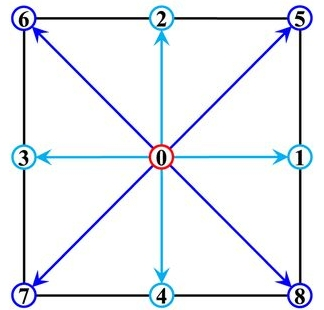
\includegraphics[scale=0.25]{images/d2q9}
\centering
\end{figure}
\end{frame}

% Discretization (velocity space): 3
\begin{frame}[t]{Discretization: velocity space}
\begin{equation*}
\left( \frac{\partial}{\partial t}
      + {\bf v}\cdot\nabla_x\right)f({\bf x}, {\bf v}, t) = \Omega(t)
\end{equation*}
The governing equation is pretty \textbf{complex} despite its seemingly simple form \\~\\

We discretize it in velocity space along \textbf{nine directions}:
\begin{figure}
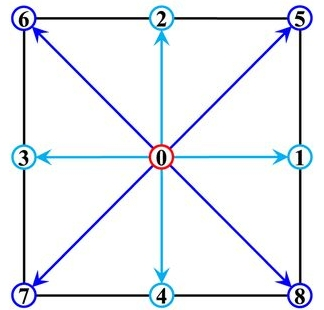
\includegraphics[scale=0.25]{images/d2q9}
\centering
\end{figure}

Which leads us to the following equation:
\begin{equation*}
\left( \frac{\partial}{\partial t}
      +  e_i \cdot\nabla_x\right)f({\bf x}, e_i, t) = \Omega(t)
\end{equation*}
where $e_i$ is a vector along each direction
\end{frame}


%-----------------------------------------------------
% Discretization (time): 1
\begin{frame}[t]{Discretization: time}
We can then discretize
\begin{equation*}
\left( \frac{\partial}{\partial t}
      +  e_i \cdot\nabla_x\right)f({\bf x}, e_i, t) = \Omega(t)
\end{equation*}
over time and write a separate expression for each $e_i$ : 
\begin{equation*}
f_i({\bf x} + e_i \delta t, t + \delta t)- f_i({\bf x}, t) = \Omega_i(t)
\end{equation*}
\end{frame}

% Discretization (time): 2
\begin{frame}[t]{Discretization: time}
We can then discretize
\begin{equation*}
\left( \frac{\partial}{\partial t}
      +  e_i \cdot\nabla_x\right)f({\bf x}, e_i, t) = \Omega(t)
\end{equation*}
over time and write a separate expression for each $e_i$ : 
\begin{equation*}
f_i({\bf x} + e_i \delta t, t + \delta t)- f_i({\bf x}, t) = \Omega_i(t)
\end{equation*}

\begin{alertblock}{Assumption}
The \textbf{collision term} $\Omega$ turns out to be \textbf{very complex} in general. It can be simplified by using a well-known and widely used assumption, the Bhatnagar-Gross-Krook (\textbf{BGK}) \cite{lattice_boltzmann_epfl} assumption. It says that the 
\textit{collision term induces the particle distribution to decay slowly to its equilibrium distribution $f^{eq}$.}

\begin{equation*}
\Omega_i = \frac{1}{\tau}\left(f_i^\text{eq} - f_i\right)
\end{equation*}
\end{alertblock}
\end{frame}


% Discretization (time): 3
\begin{frame}[t]{Discretization: time}
\begin{itemize}
\item The equilibrium distribution is \textbf{a smoothed version of the current distribution}, recomputed from the bulk properties $\rho$ and $\textbf{u}$ (bulk velocity) \cite{lattice_boltzmann}. \\~\\

\item The equilibrium represents \textbf{an expected distribution} which would result in the observed bulk properties \cite{lattice_boltzmann}. \\~\\

\item According to \textbf{the BGK assumption}, the equilibrium distribution can be represented by the following: 

\end{itemize}
\end{frame}

% Discretization (time): 4
\begin{frame}[t]{Discretization: time}
\begin{itemize}
\item The equilibrium distribution is \textbf{a smoothed version of the current distribution}, recomputed from the bulk properties $\rho$ and $\textbf{u}$ (bulk velocity) \cite{lattice_boltzmann}. \\~\\

\item The equilibrium represents \textbf{an expected distribution} which would result in the observed bulk properties \cite{lattice_boltzmann}. \\~\\

\item According to \textbf{the BGK assumption}, the equilibrium distribution can be represented by the following:
\end{itemize}

\begin{equation*}
f_i^\text{eq} = \omega_i \rho \left(1 + 3\frac{e_i \cdot u}{c} + \frac92 \frac{(e_i \cdot u)^2}{c^2} - \frac32 \frac{u\cdot u}{c^2}\right)
\end{equation*}
where $\omega_i$ - a weighting function dependent on the exact velocity discretization; $c = \frac{1}{\sqrt{3}}$ - the \textit{lattice} speed of sound 
\end{frame}
%%%%%%%%%%%%%%%%%%%%%%%%%%%%%%%%%%%%%%%%%%%%%%%%%%%%%%
% Mesoscopic to Macroscopic: 1
\subsection{From Mesoscopic to Macroscopic}
\begin{frame}[t]{Jump from Mesoscopic to Macroscopic World}
Let's take a closer look at the equilibrium distribution equation
\begin{equation*}
f_i^\text{eq} = \omega_i \rho \left(1 + 3\frac{e_i \cdot u}{c} + \frac92 \frac{(e_i \cdot u)^2}{c^2} - \frac32 \frac{u\cdot u}{c^2}\right)
\end{equation*}
To compute this equation, we need to know the bulk \textbf{density} and the \textbf{velocity} 
\end{frame}

% Mesoscopic to Macroscopic: 2
\begin{frame}[t]{Jump from Mesoscopic to Macroscopic World}
Let's take a closer look at the equilibrium distribution equation
\begin{equation*}
f_i^\text{eq} = \omega_i \rho \left(1 + 3\frac{e_i \cdot u}{c} + \frac92 \frac{(e_i \cdot u)^2}{c^2} - \frac32 \frac{u\cdot u}{c^2}\right)
\end{equation*}
To compute this equation, we need to know the bulk \textbf{density} and the \textbf{velocity} \\~\\

These can be computed as follows:

\begin{equation*}
\rho(x, t) = \sum_{i=1}^{9}{f_i}(x, t)
\end{equation*}

\begin{equation*}
\rho(x, t)\vec{u}(x, t) = \sum_{i=1}^{9}\vec{e}_i{f_i}(x, t)
\end{equation*}
\end{frame}

% Mesoscopic to Macroscopic: 3
\begin{frame}[t]{Jump from Mesoscopic to Macroscopic World}
Let's take a closer look at the equilibrium distribution equation:
\begin{equation*}
f_i^\text{eq} = \omega_i \rho \left(1 + 3\frac{e_i \cdot u}{c} + \frac92 \frac{(e_i \cdot u)^2}{c^2} - \frac32 \frac{u\cdot u}{c^2}\right)
\end{equation*}
To compute this equation, we need to know the bulk \textbf{density} and the \textbf{velocity} \\~\\

These can be computed as follows:

\begin{equation*}
\rho(x, t) = \sum_{i=1}^{9}{f_i}(x, t)
\end{equation*}

\begin{equation*}
\rho(x, t)\vec{u}(x, t) = \sum_{i=1}^{9}\vec{e}_i{f_i}(x, t)
\end{equation*}
\begin{alertblock}{IMPORTANT!}
\begin{itemize}
\item
All equation above are dimensionless.
\item
One has to use \textbf{scaling} to simulate a real liquid.
\end{itemize}
\end{alertblock}
\end{frame}

%%%%%%%%%%%%%%%%%%%%%%%%%%%%%%%%%%%%%%%%%%%%%%%%%%%%%%
% LBM "Pipeline": 1
\subsection{LBM "Pipeline"}
\begin{frame}[t]{All together}
The discretized governing equation
\begin{equation*}
f_i({\bf x} + e_i \delta t, t + \delta t)- f_i({\bf x}, t) = \Omega_i(t)
\end{equation*}
along with the collision operator
\begin{equation*}
\Omega_i = \frac{1}{\tau}\left(f_i^\text{eq}(\rho({\bf x}, t), u({\bf x}, t)) - f_i({\bf x}, t)\right)
\end{equation*}
where the equilibrium distribution equation has the following form:
\begin{equation*}
f_i^\text{eq} = \omega_i \rho \left(1 + 3\frac{e_i \cdot u}{c} + \frac92 \frac{(e_i \cdot u)^2}{c^2} - \frac32 \frac{u\cdot u}{c^2}\right)
\end{equation*}
give us \textbf{the final equation} for each \textbf{direction $i$ }: 
\end{frame}


% LBM "Pipeline": 2
\begin{frame}[t]{All together}
The discretized governing equation
\begin{equation*}
f_i({\bf x} + e_i \delta t, t + \delta t)- f_i({\bf x}, t) = \Omega_i(t)
\end{equation*}
along with the collision operator
\begin{equation*}
\Omega_i = \frac{1}{\tau}\left(f_i^\text{eq}(\rho({\bf x}, t), u({\bf x}, t)) - f_i({\bf x}, t)\right)
\end{equation*}
where the equilibrium distribution equation has the following form:
\begin{equation*}
f_i^\text{eq} = \omega_i \rho \left(1 + 3\frac{e_i \cdot u}{c} + \frac92 \frac{(e_i \cdot u)^2}{c^2} - \frac32 \frac{u\cdot u}{c^2}\right)
\end{equation*}
give us \textbf{the final equation} for each \textbf{direction $i$ }:

\begin{equation*}
f_i({\bf x} + e_i \delta t, t + \delta t) = f_i({\bf x}, t) - \frac{1}{\tau}\left(f_i({\bf x}, t) - f_i^\text{eq}(\rho({\bf x}, t), u({\bf x}, t))\right)
\end{equation*}
\end{frame}


% LBM "Pipeline": 3
\begin{frame}[t]{Pipeline}
If you look at the final equation
\begin{equation*}
f_i({\bf x} + e_i \delta t, t + \delta t) = f_i({\bf x}, t) - \frac{1}{\tau}\left(f_i({\bf x}, t) - f_i^\text{eq}(\rho({\bf x}, t), u({\bf x}, t))\right)
\end{equation*}
you can easily find two distinct steps, namely:
\end{frame}

% LBM "Pipeline": 3
\begin{frame}[t]{Pipeline}
If you look at the final equation
\begin{equation*}
f_i({\bf x} + e_i \delta t, t + \delta t) = f_i({\bf x}, t) - \frac{1}{\tau}\left(f_i({\bf x}, t) - f_i^\text{eq}(\rho({\bf x}, t), u({\bf x}, t))\right)
\end{equation*}
you can easily find two distinct steps, namely:

\textbf{Collision}:
\begin{equation*}
f_i({\bf x}, t)^* = f_i({\bf x}, t) - \frac{1}{\tau}\left(f_i({\bf x}, t) - f_i^\text{eq}(\rho({\bf x}, t), u({\bf x}, t))\right)
\end{equation*}
\end{frame}

% LBM "Pipeline": 4
\begin{frame}[t]{Pipeline}
Looking at the final equations
\begin{equation*}
f_i({\bf x} + e_i \delta t, t + \delta t) = f_i({\bf x}, t) - \frac{1}{\tau}\left(f_i({\bf x}, t) - f_i^\text{eq}(\rho({\bf x}, t), u({\bf x}, t))\right)
\end{equation*}
Once can easily find two distinct steps, namely: \\~\\
\textbf{Collision}:
\begin{equation*}
f_i({\bf x}, t)^* = f_i({\bf x}, t) - \frac{1}{\tau}\left(f_i({\bf x}, t) - f_i^\text{eq}(\rho({\bf x}, t), u({\bf x}, t))\right)
\end{equation*}
\\~\\
\textbf{Streaming}:
\begin{equation*}
f_i({\bf x} + e_i \delta t, t + \delta t) = f_i({\bf x}, t)^*
\end{equation*}
\end{frame}


% LBM "Pipeline": 5
\begin{frame}[t]{Pipeline}
\textbf{Collision}:
\begin{equation*}
f_i({\bf x}, t)^* = f_i({\bf x}, t) - \frac{1}{\tau}\left(f_i({\bf x}, t) - f_i^\text{eq}(\rho({\bf x}, t), u({\bf x}, t))\right)
\end{equation*}
\\~\\
\textbf{Streaming}:
\begin{equation*}
f_i({\bf x} + e_i \delta t, t + \delta t) = f_i({\bf x}, t)^*
\end{equation*}

\begin{figure}
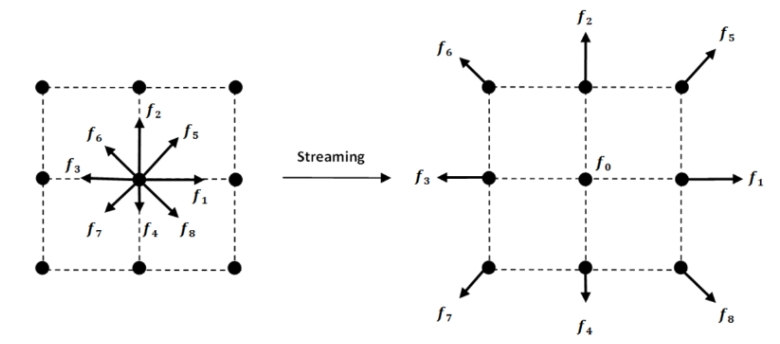
\includegraphics[scale=0.25]{images/collistion-streaming.jpg}
\centering
\end{figure}
\end{frame}

% LBM "Pipeline": 6
\begin{frame}[t]{Pipeline}
\textbf{Collision}:
\begin{equation*}
f_i({\bf x}, t)^* = f_i({\bf x}, t) - \frac{1}{\tau}\left(f_i({\bf x}, t) - f_i^\text{eq}(\rho({\bf x}, t), u({\bf x}, t))\right)
\end{equation*}
\\~\\
\textbf{Streaming}:
\begin{equation*}
f_i({\bf x} + e_i \delta t, t + \delta t) = f_i({\bf x}, t)^*
\end{equation*}

\begin{figure}
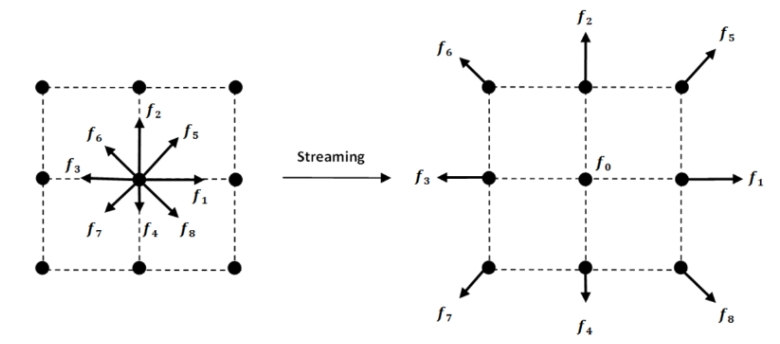
\includegraphics[scale=0.25]{images/collistion-streaming.jpg}
\centering
\end{figure}

\begin{block}{NOTE:}
One can easily rewrite \textbf{collision-streaming} steps as \textbf{streaming-collision} ones
\end{block}
\end{frame}
%%%%%%%%%%%%%%%%%%%%%%%%%%%%%%%%%%%%%%%%%%%%%%%%%%%%%%
% Boundary conditions : 1
\subsection{Boundary conditions}
\begin{frame}[t]{Boundary conditions}
We want to simulate a wind tunnel with an arbitrary object inside
\\~\\
\begin{figure}
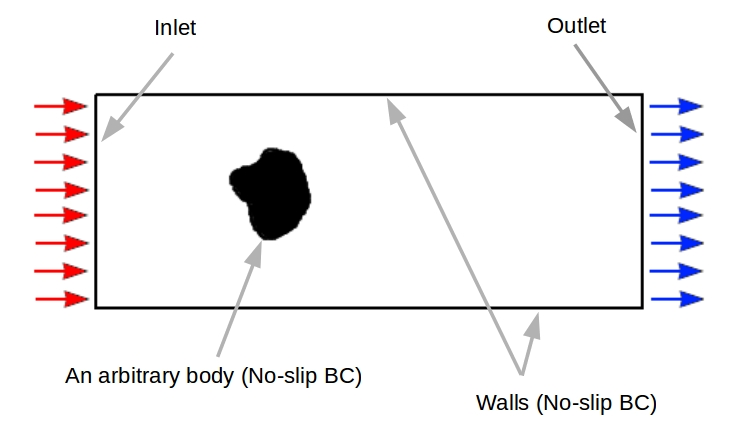
\includegraphics[scale=0.35]{images/wind-tunnel.jpg}
\centering
\end{figure}
\textbf{But ...}
\end{frame}

% Boundary conditions : 2
\begin{frame}[t]{Boundary conditions}
We want to simulate a wind tunnel with an arbitrary object inside
\\~\\
\begin{figure}
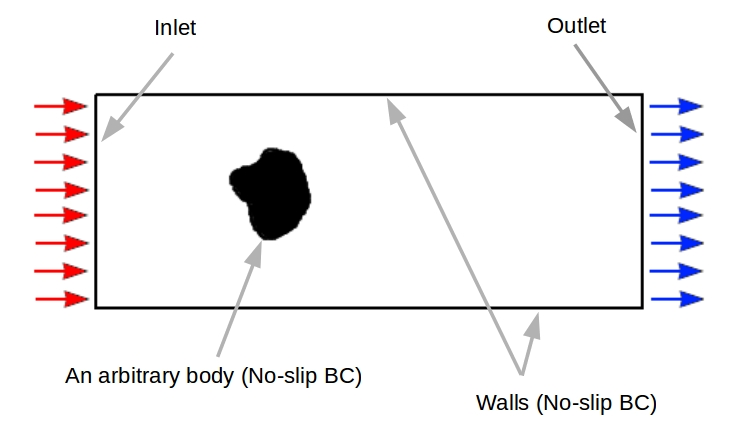
\includegraphics[scale=0.35]{images/wind-tunnel.jpg}
\centering
\end{figure}
\textbf{The last piece} of LBM theory that we have not discussed yet is the \textbf{Boundary Conditions} and their implementation
\end{frame}


% Boundary conditions : 3
\begin{frame}[t]{Boundary conditions}
\begin{itemize}
\item There is a whole "zoo" of boundary conditions for Lattice Boltzmann.
\end{itemize}
\end{frame}
 
% Boundary conditions : 4
\begin{frame}[t]{Boundary conditions}
\begin{itemize}
\item There is a whole "zoo" of boundary conditions for Lattice Boltzmann.
\\~\\
\item Each implementation has its advantages and disadvantages (\textit{\textbf{e.g.}, accuracy vs programming complexity})
\end{itemize}
\end{frame}

% Boundary conditions : 5
\begin{frame}[t]{Boundary conditions}
\begin{itemize}
\item There is a whole "zoo" of boundary conditions for Lattice Boltzmann.
\\~\\
\item Each implementation has its advantages and disadvantages (\textit{\textbf{e.g.}, accuracy vs programming complexity}.)
\\~\\
\item We are going to demonstrate an implementation of the \textbf{"non-slip"} (so-called \textbf{bounce back}) boundary conditions to show you how they work.
\end{itemize}
\end{frame}

% Boundary conditions : 6
\begin{frame}[t]{Boundary conditions}
\begin{itemize}
\item There is a whole "zoo" of boundary conditions for Lattice Boltzmann.
\\~\\
\item Each implementation has its advantages and disadvantages (\textit{\textbf{e.g.}, accuracy vs programming complexity}.)
\\~\\
\item We are going to demonstrate an implementation of the \textbf{"non-slip"} (so-called \textbf{bounce back}) boundary conditions to show you how they work.
\\~\\
\item Please, read corresponding literature to get an idea of how different boundary conditions can be implemented.
\end{itemize}
\end{frame}

% Boundary conditions : 7
\begin{frame}[t]{Bounce Back BC}
\begin{figure}
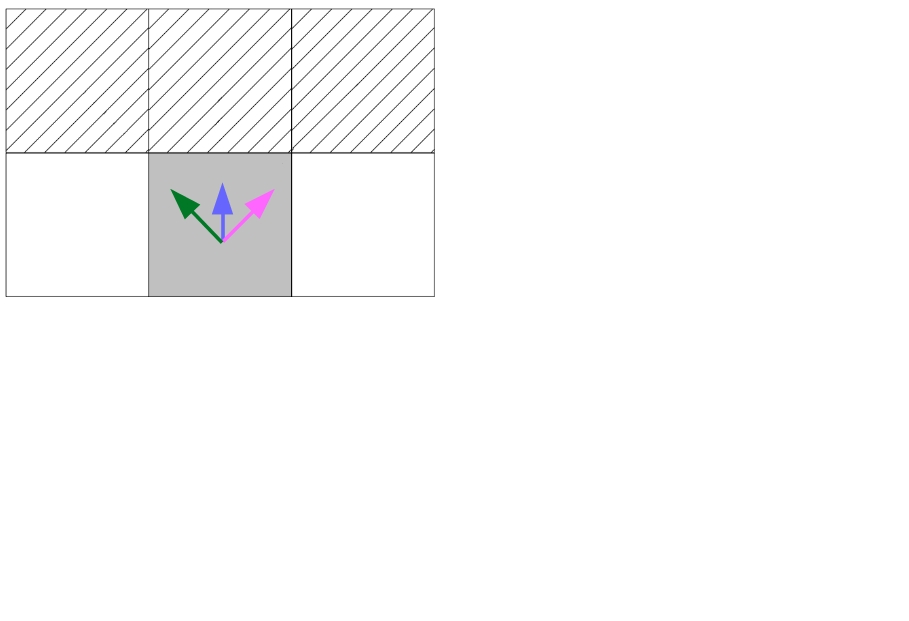
\includegraphics[scale=0.3]{images/bounce-back-bc-1.jpg}
\centering
\end{figure}
\end{frame}

% Boundary conditions : 8
\begin{frame}[t]{Bounce Back BC}
\begin{figure}
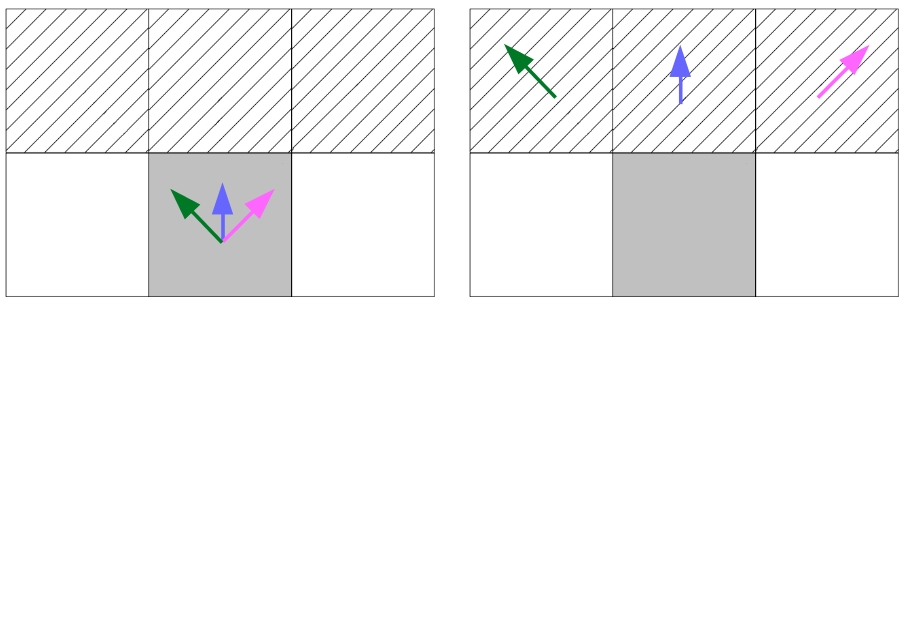
\includegraphics[scale=0.3]{images/bounce-back-bc-2.jpg}
\centering
\end{figure}
\end{frame}

% Boundary conditions : 9
\begin{frame}[t]{Bounce Back BC}
\begin{figure}
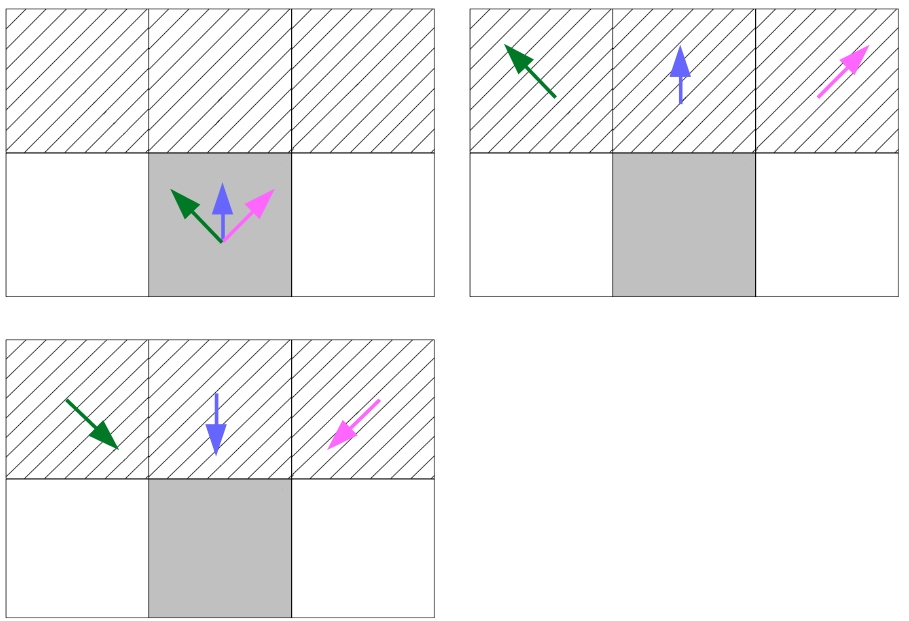
\includegraphics[scale=0.3]{images/bounce-back-bc-3.jpg}
\centering
\end{figure}
\end{frame}

% Boundary conditions : 10
\begin{frame}[t]{Bounce Back BC}
\begin{figure}
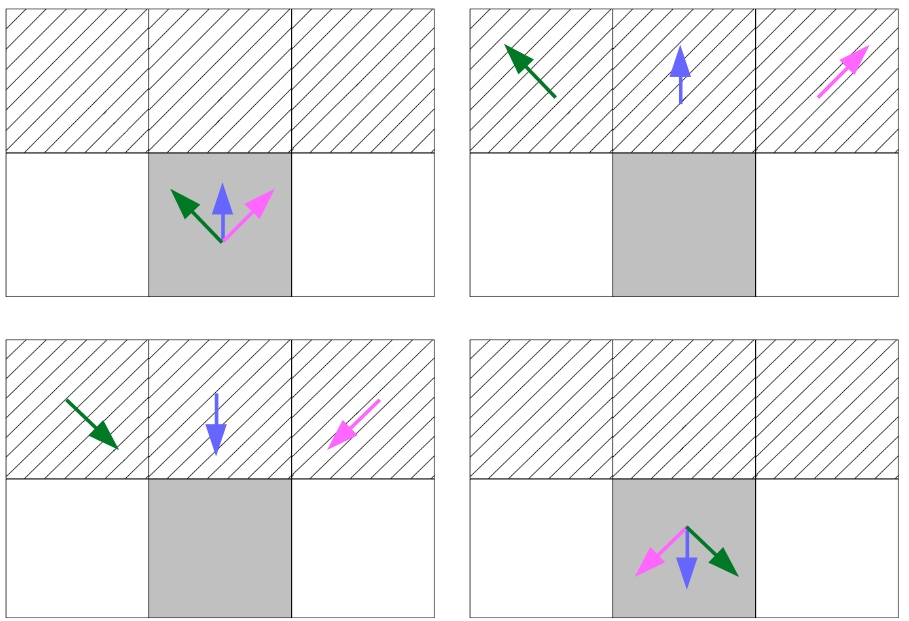
\includegraphics[scale=0.3]{images/bounce-back-bc-4.jpg}
\centering
\end{figure}
\end{frame}

% Boundary conditions : 11
\begin{frame}[t]{LBM Algorithmic Properties}
\emphasize{Advantages:}
\begin{itemize}
\item LBM with BKG assumptions is easy to implement
\item Streaming and Collision are \textbf{embarrassingly parallel} steps
\item It is a \textbf{matrix free} method (no need to store the entire matrix)
\begin{itemize}
	\item equations are built on the fly
\end{itemize}

\end{itemize}

\end{frame}

% Boundary conditions : 12
\begin{frame}[t]{LBM Algorithmic Properties}
\emphasize{Advantages:}
\begin{itemize}
\item LBM with BKG assumptions is easy to implement
\item Streaming and Collision are \textbf{embarrassingly parallel} steps
\item It is a \textbf{matrix free} method (no need to store the entire matrix)
\begin{itemize}
	\item equations are built on the fly
\end{itemize}

\end{itemize}
\emphasize{Disadvantages:}
\begin{itemize}
\item The algorithm is \textbf{memory bound}
\end{itemize}
\end{frame}


% Boundary conditions : 13
\begin{frame}[t]{LBM Algorithmic Properties}
\emphasize{Advantages:}
\begin{itemize}
\item LBM with BKG assumptions is easy to implement
\item Streaming and Collision are \textbf{embarrassingly parallel} steps
\item It is a \textbf{matrix free} method (no need to store the entire matrix)
\begin{itemize}
	\item equations are built on the fly
\end{itemize}

\end{itemize}
\emphasize{Disadvantages:}
\begin{itemize}
\item The algorithm is \textbf{memory bound}
\item The streaming step does not have any computational load. It \textbf{just moves data} from one place to another. Hence, it creates huge memory traffic.
\end{itemize}
\end{frame}

% Boundary conditions : 14
\begin{frame}[t]{LBM Algorithmic Properties}
\emphasize{Advantages:}
\begin{itemize}
\item LBM with BKG assumptions is easy to implement.
\item Streaming and Collision are \textbf{embarrassingly parallel} steps.
\item It is a \textbf{matrix free} method (no need to store the entire matrix).
\begin{itemize}
	\item equations are built on the fly
\end{itemize}

\end{itemize}
\emphasize{Disadvantages:}
\begin{itemize}
\item The algorithm is \textbf{memory bound}
\item The streaming step does not have any computational load. It \textbf{just moves data} from one place to another. Hence, it creates huge memory traffic.
\item To build an equation on the fly, we have to differentiate between elements according to their types. Thus, we need to assign \textbf{a flag to each element}. Hence, we have to hold and process an additional data structure.
\end{itemize}
\end{frame}


% Boundary conditions : 15
\begin{frame}[t]{LBM Algorithmic Properties}
\emphasize{Advantages:}
\begin{itemize}
\item LBM with BKG assumptions is easy to implement
\item Streaming and Collision are \textbf{embarrassingly parallel} steps
\item It is a \textbf{matrix free} method (no need to store the entire matrix)
\begin{itemize}
	\item equations are built on the fly
\end{itemize}

\end{itemize}
\emphasize{Disadvantages:}
\begin{itemize}
\item The algorithm is \textbf{memory bound}
\item The streaming step does not have any computational load. It \textbf{just moves data} from one place to another. Hence, it creates huge memory traffic.
\item To build an equation on the fly, we have to differentiate between elements according to their types. Thus, we need to assign \textbf{a flag to each element}. Hence, we have to hold and process additional data structure.
\begin{alertblock}{Note}
We have to \textbf{check flags} for each neighboring element to build the right equation \textbf{in each iteration}. This leads to a \textbf{huge ladder of if-else statements} which lead to \textbf{branch divergence} on the GPU.
\end{alertblock}

\end{itemize}
\end{frame}


% Boundary conditions : 16
\begin{frame}[t]{Improvement of LBM Algorithmic Properties}
\begin{block}{Disadvantages}
We have to \textbf{check flags} for each neighboring element to build the right equation \textbf{in each iteration}. This leads to a \textbf{huge ladder of if-else statements} which lead to \textbf{branch divergence} on the GPU.
\end{block}
\begin{itemize}
\item Perform \textbf{functional decomposition} before the main loop.
\end{itemize}
\end{frame}


% Boundary conditions : 17
\begin{frame}[t]{Improvement of LBM Algorithmic Properties}
\begin{block}{Disadvantages}
We have to \textbf{check flags} for each neighboring element to build the right equation \textbf{in each iteration}. This leads to a \textbf{huge ladder of if-else statements} which lead to \textbf{branch divergence} on the GPU.
\end{block}
\begin{itemize}
\item Perform \textbf{functional decomposition} before the main loop.
\item Update elements of the \textbf{same type} separately.
\end{itemize}
\end{frame}



% Boundary conditions : 18
\begin{frame}[t]{Improvement of LBM Algorithmic Properties}
\begin{block}{Disadvantages}
We have to \textbf{check flags} for each neighboring element to build the right equation \textbf{in each iteration}. This leads to a \textbf{huge ladder of if-else statements} which lead to \textbf{branch divergence} on the GPU.
\end{block}
\begin{itemize}
\item Perform \textbf{functional decomposition} before the main loop.
\item Update elements of the \textbf{same type} separately.
\item In other words, remember \textbf{where, what and how} to update.
\end{itemize}
\end{frame}



% Boundary conditions : 19
\begin{frame}[t]{Improvement of LBM Algorithmic Properties}
\begin{block}{Disadvantages}
We have to \textbf{check flags} for each neighboring element to build the right equation \textbf{in each iteration}. This leads to a \textbf{huge ladder of if-else statements} which lead to \textbf{branch divergence} on the GPU.
\end{block}
\begin{itemize}
\item Perform \textbf{functional decomposition} before the main loop.
\item Update elements of the \textbf{same type} separately.\
\item In other words, remember \textbf{where, what and how} to update.
\item Put elements of the same type in a \textbf{separate data structure}.
\end{itemize}
\end{frame}


% Boundary conditions : 20
\begin{frame}[t]{Scanning}
\begin{figure}
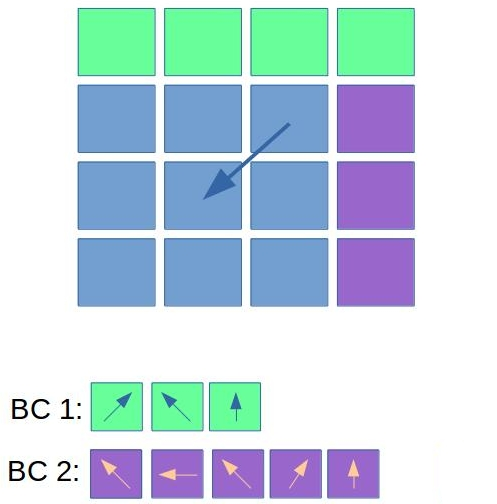
\includegraphics[scale=0.3]{images/scan-1.jpg}
\centering
\end{figure}
\end{frame}

% Boundary conditions : 21
\begin{frame}[t]{Scanning}
\begin{figure}
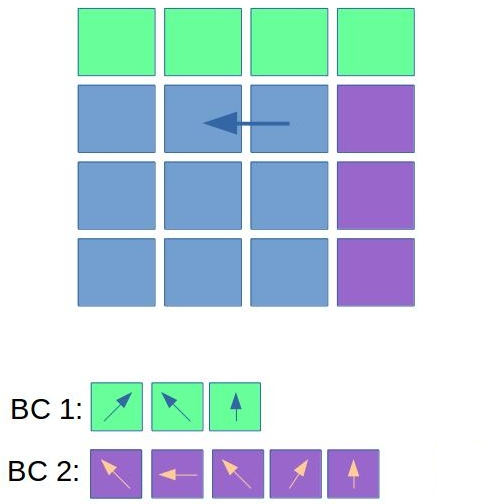
\includegraphics[scale=0.3]{images/scan-2.jpg}
\centering
\end{figure}
\end{frame}

% Boundary conditions : 22
\begin{frame}[t]{Scanning}
\begin{figure}
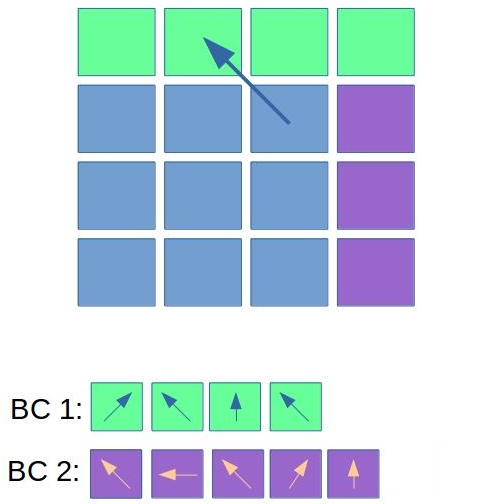
\includegraphics[scale=0.3]{images/scan-3.jpg}
\centering
\end{figure}
\end{frame}

% Boundary conditions : 23
\begin{frame}[t]{Scanning}
\begin{figure}
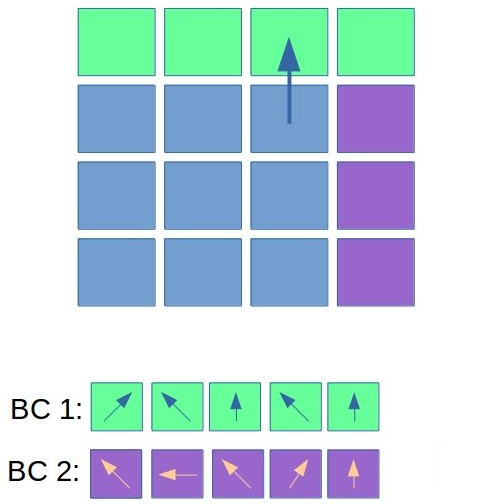
\includegraphics[scale=0.3]{images/scan-4.jpg}
\centering
\end{figure}
\end{frame}

% Boundary conditions : 24
\begin{frame}[t]{Scanning}
\begin{figure}
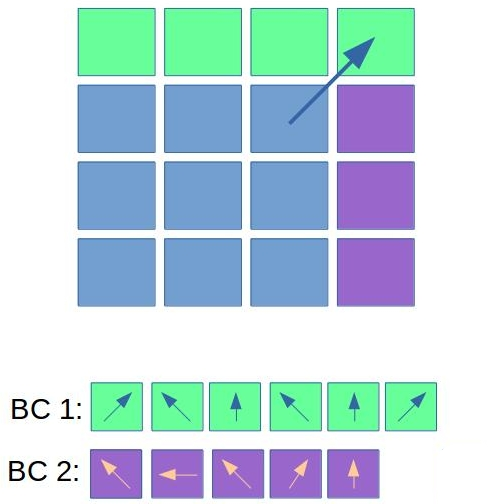
\includegraphics[scale=0.3]{images/scan-5.jpg}
\centering
\end{figure}
\end{frame}

% Boundary conditions : 25
\begin{frame}[t]{Scanning}
\begin{figure}
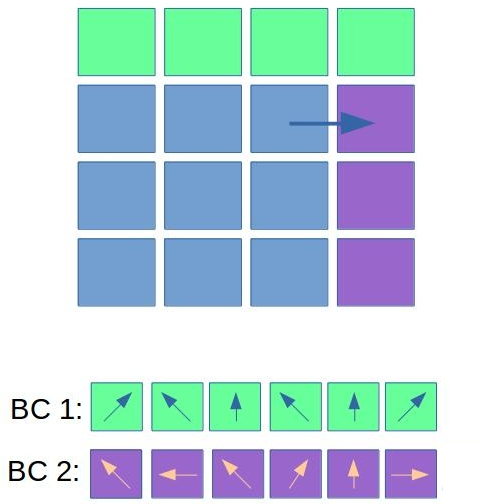
\includegraphics[scale=0.3]{images/scan-6.jpg}
\centering
\end{figure}
\end{frame}

% Boundary conditions : 26
\begin{frame}[t]{Scanning}
\begin{figure}
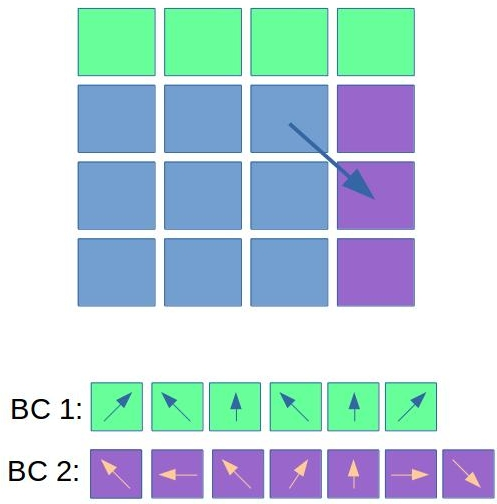
\includegraphics[scale=0.3]{images/scan-7.jpg}
\centering
\end{figure}
\end{frame}

% Boundary conditions : 27
\begin{frame}[t]{Scanning}
\begin{figure}
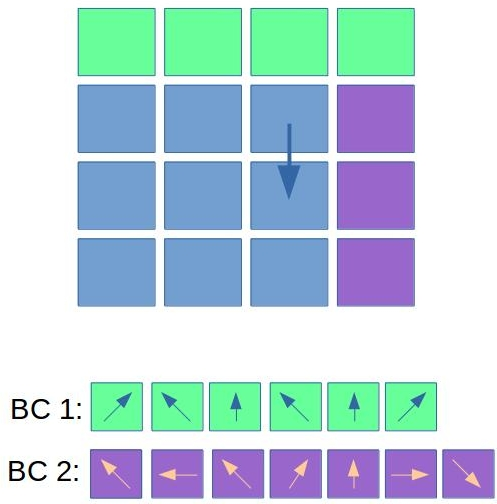
\includegraphics[scale=0.3]{images/scan-8.jpg}
\centering
\end{figure}
\end{frame}
%%%%%%%%%%%%%%%%%%%%%%%%%%%%%%%%%%%%%%%%%%%%%%%%%%%%%%
% Example : 1
\section{Results}
\begin{frame}{Simulations and all that}

\centering 
\huge Time for some videos.

\end{frame}

%%%%%%%%%%%%%%%%%%%%%%%%%%%%%%%%%%%%%%%%%%%%%%%%%%%%%%
%%%%%%%%%%%%%%%%%%%%%%%%%%%%%%%%%%%%%%%%%%%%%%%%%%%%%%%%%%%%%%%%%%%%%%%%%%%%%%
\section{Performance}
%---------------- Performance on different GPUs ----------------------------

\begin{frame}{Performance on GPUs}
We ran the application on a number of different GPUs. 

\begin{figure}
\begin{center}
	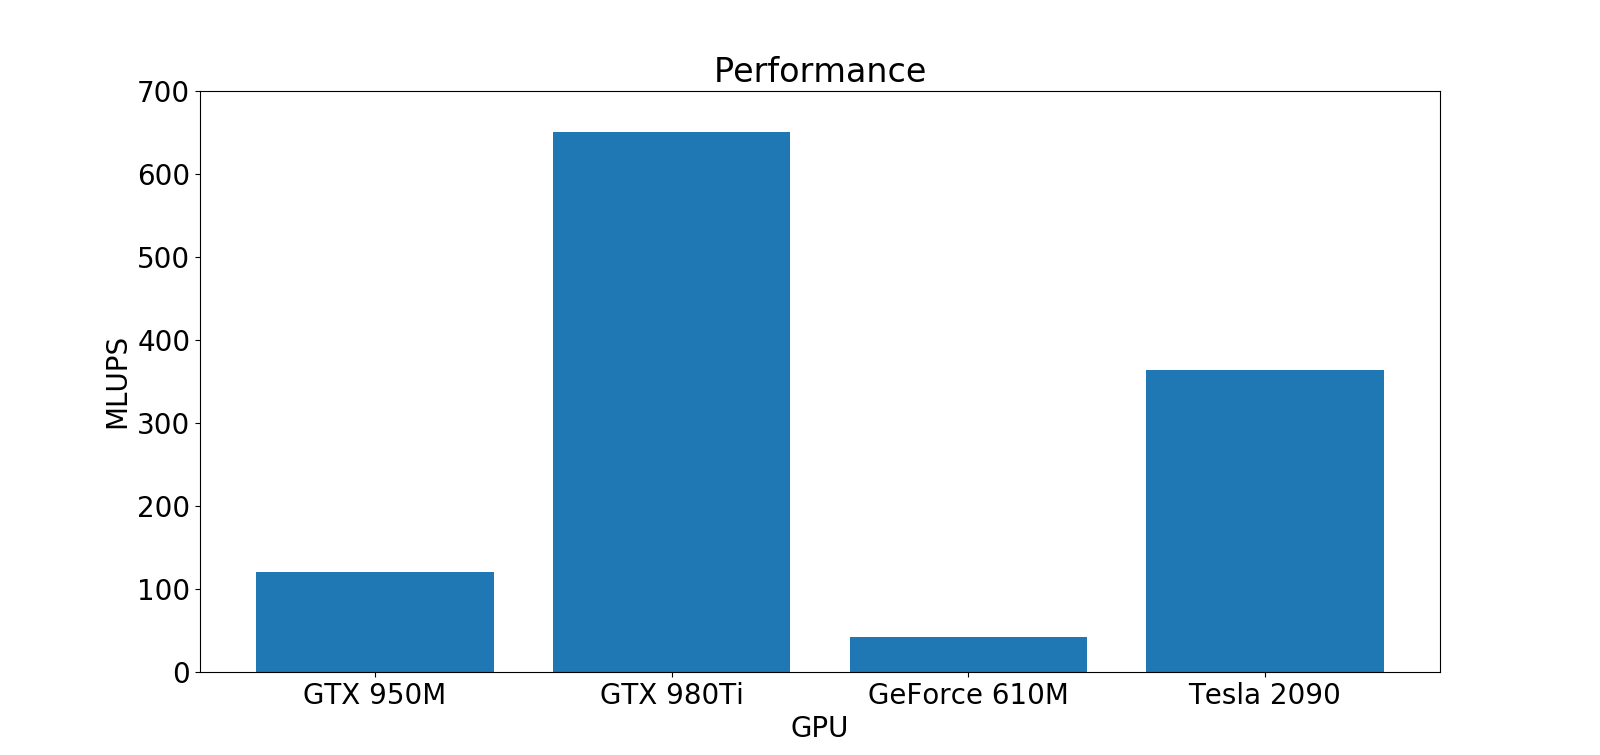
\includegraphics[scale=0.25]{images/performance_on_different_gpus.png}
\end{center}
\end{figure}

\end{frame}


%-----------------------Performance correlation------------------------------

\begin{frame}{Core-Performance correlation}
How do you think the core count is correlated with the performance? 
\pause 

\begin{figure}
\begin{center}
	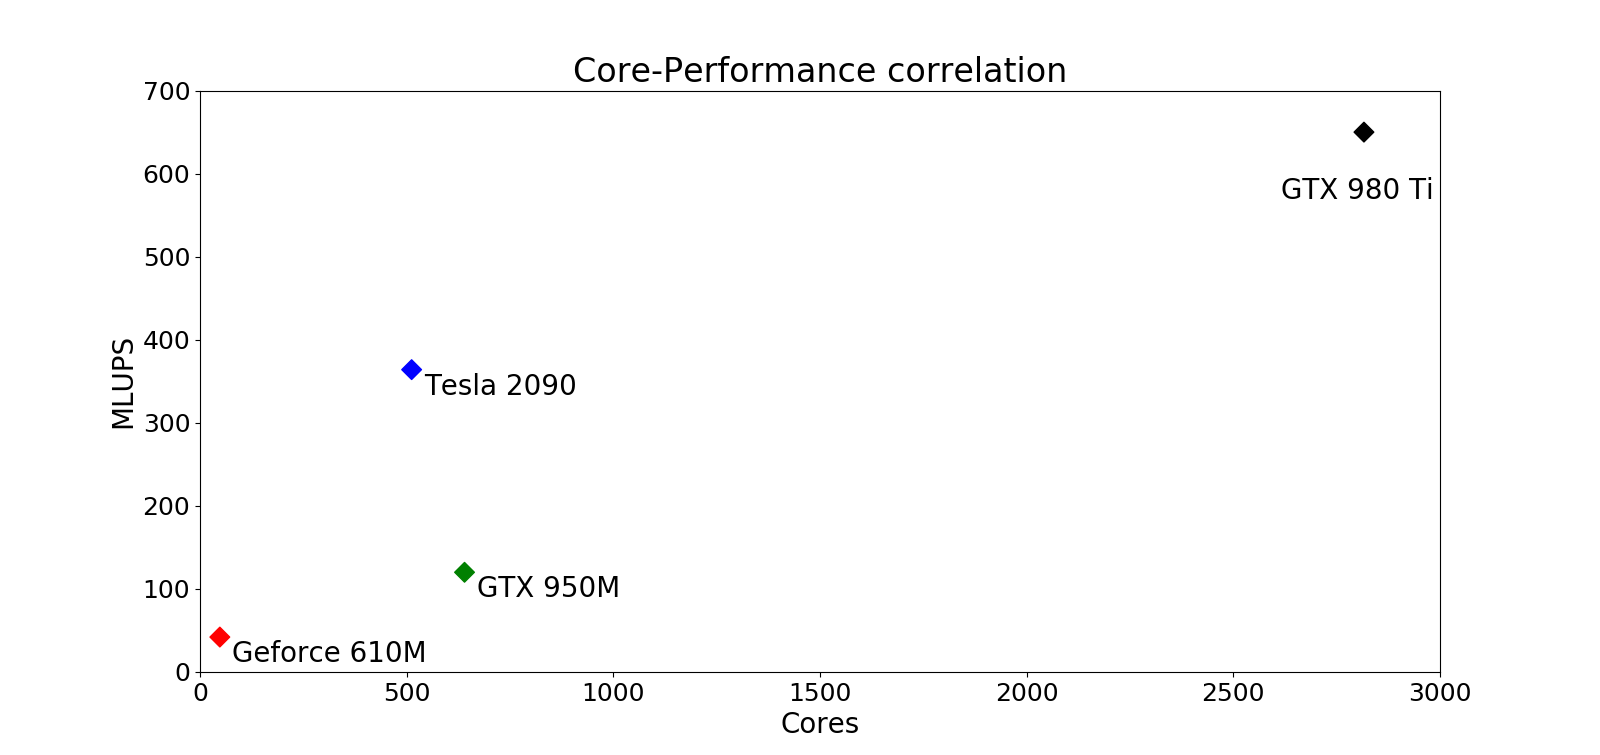
\includegraphics[scale=0.25]{images/core_mlups.png}
\end{center}
\end{figure}
\end{frame}

\begin{frame}{Bandwidth-Performance correlation}
What about the \textbf{bandwidth?} \\
\pause
\begin{figure}
\begin{center}
	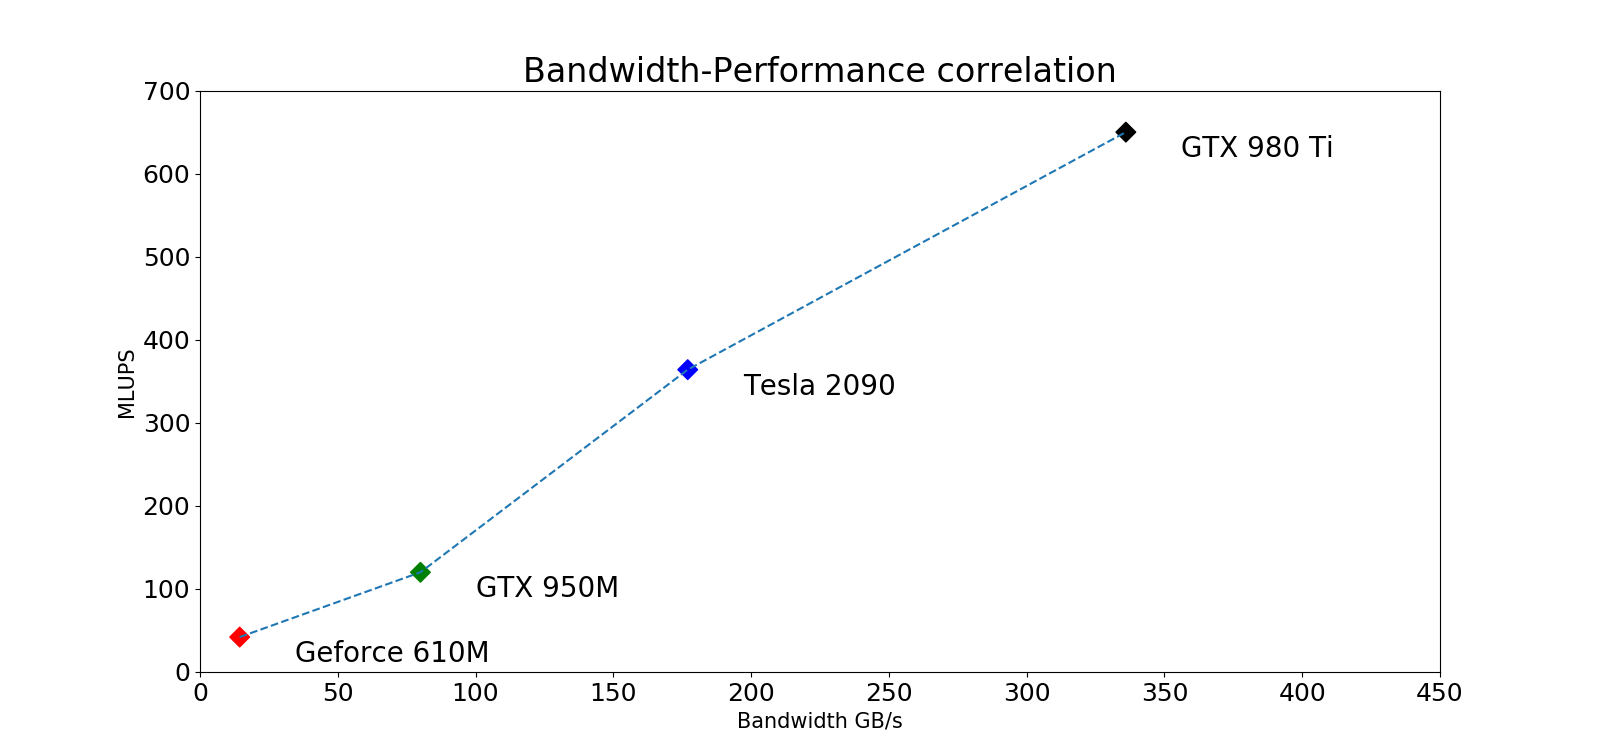
\includegraphics[scale=0.25]{images/bandwidth_mlups_corr.png}
\end{center}
\end{figure}
\end{frame}

\begin{frame}{Frequency-Performance correlation}
Let us take a look at frequency too. 
\begin{figure}
\begin{center}
	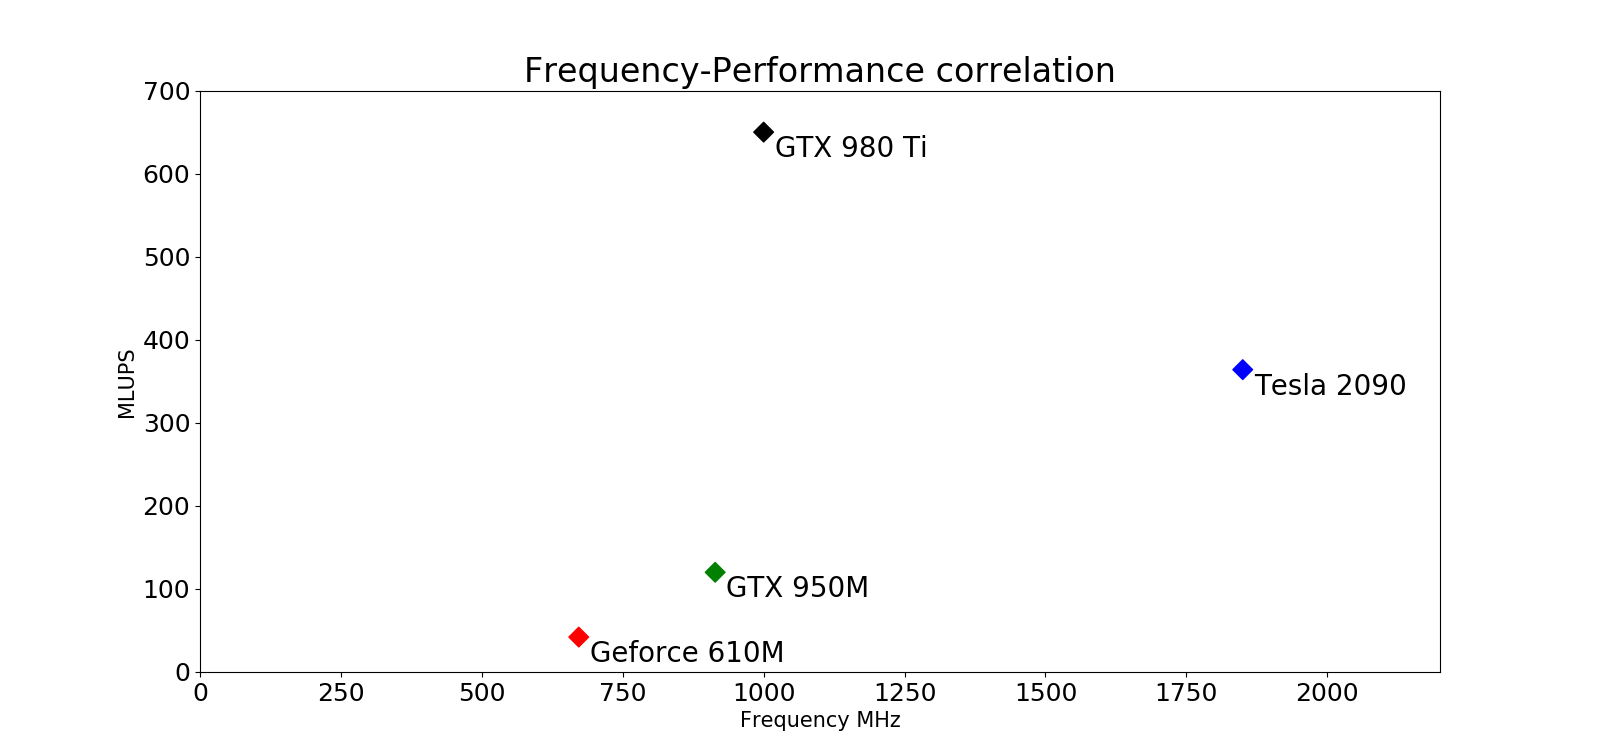
\includegraphics[scale=0.25]{images/freq_mlups_corr.png}
\end{center}
\end{figure}
\end{frame}


%%%%%%%%%%%%%%%%%%%%%%%%%%%%%%%%%%%%%%%%%%%%%%%%%%%%%%

% Memory / Optimization 
% TODO: Does it make sense to talk about optimization here? 
% TODO: This seems to be just about the memory. 
\section{CUDA Optimization and Memory}

%ref [2h]
\begin{frame}{General Steps Towards Optimization}
Some general principles for optimization:
\begin{columns}

\begin{column}{0.5\textwidth}
\begin{itemize}

	\item Minimize host-device memory interactions.
    \medskip
	
    \item Use coalesced memory access. 
    \medskip
    
    \item Set kernel execution parameters to achieve higher occupancy. 

  

\end{itemize}

\pause

\end{column}

\begin{column}{0.5\textwidth}
\begin{itemize}
    \item Pay attention to register and shared memory usage. 
    
    \medskip
    \item Divergent code can significantly reduce performance. In the worst case, by a factor of 32.  	
\end{itemize}
\end{column}

\end{columns}
\end{frame}

%------------------------------Memory Hierarchy-----------------------------------
\begin{frame}{Memory Hierarchy}


\begin{itemize}

	\item  CPUs have low bandwidth and hide latency through caching
    
    \item GPUs have higher bandwidth but also higher latency: 400 - 800 cycles  

\end{itemize}
\pause
\begin{figure}
\begin{center}
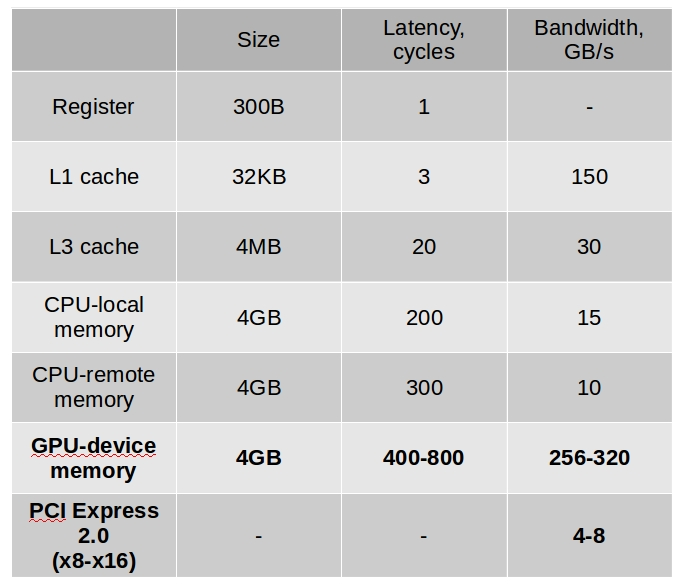
\includegraphics[scale=0.3]{images/latency-bandwidth.jpg}
\end{center}
\end{figure}

\end{frame}

%------------- Memory and compute bound applications ---------------------

\begin{frame}[t]{Memory and Computational Limitations}
\begin{columns}

\begin{column}{0.5\textwidth}
An application can be either memory or compute bounded. 
\begin{itemize}
	\item Memory bounded - Not enough bandwidth to utilize all FPUs.
	\item Compute bounded - All FPUs are occupied but we have more data available. 
\end{itemize}

\bigskip
\pause

A simple heuristic for determining memory boundedness: 

\begin{itemize}
	\item Switch from double to float. 
    \item Memory bounded if speedup is small - for example 2. 
\end{itemize}

\end{column}

\pause

\begin{column}{0.5\textwidth}
\begin{center}

%ref: [1h]
\begin{tabular}{|c|c|c|c|}
\hline
Compute Capability & 3.0 & 5.0, 5.2 & \color{red} 6.0 \\
\hline
Float Throughput & 192 & 128 & \color{red} 64  \\
\hline
Double Throughput & 8 & 4 & \color{red} 32 \\
\hline
Ratio & 24 & 32 & \color{red} 2\\
\hline
\end{tabular}

\bigskip
\bigskip

\begin{figure}
\begin{center}
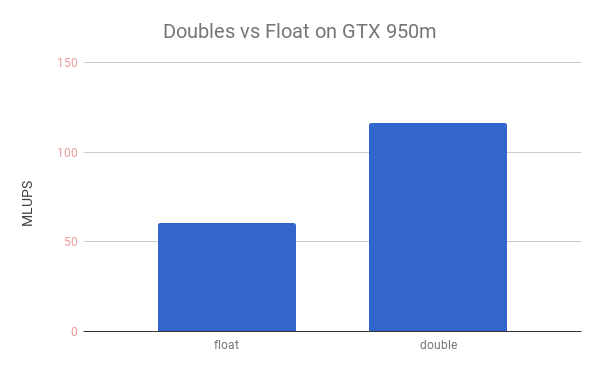
\includegraphics[scale=0.25]{images/doubles_vs_floats.png}
\end{center}
\end{figure}

\end{center}
\end{column}

\end{columns}
\end{frame}

%------------ Host - Device Memory interactions in our code--------------------
\begin{frame}[t]{Host - Device Memory Interactions}

Since data transfers between the CPU and GPU are limited by the PCIe bus, our code only requires host-device memory interactions in the beginning. Thereafter, GPU computations do not require memory interactions with the CPU. 

\begin{figure}
\begin{center}
\includegraphics[width=0.6\textwidth]{images/transferless_algorithm.png}
\end{center}
\end{figure}

\end{frame}

%%%%%%%%%%%%%%%%%%%%%%%%%%%%%%%%%%%%%%%%%%%%%%%%%%%%%%
%Coalesced Memory Access
\section{Coalesced Memory Access}

%What is coalesced memory access? 
\begin{frame}[t]{What is coalesced memory access?}
If threads in a warp access nearby memory locations then these memory requests can be \textbf{coalesced} into fewer transactions \cite{nv_prog_guide}. 

\bigskip 

\begin{figure}
\begin{center}
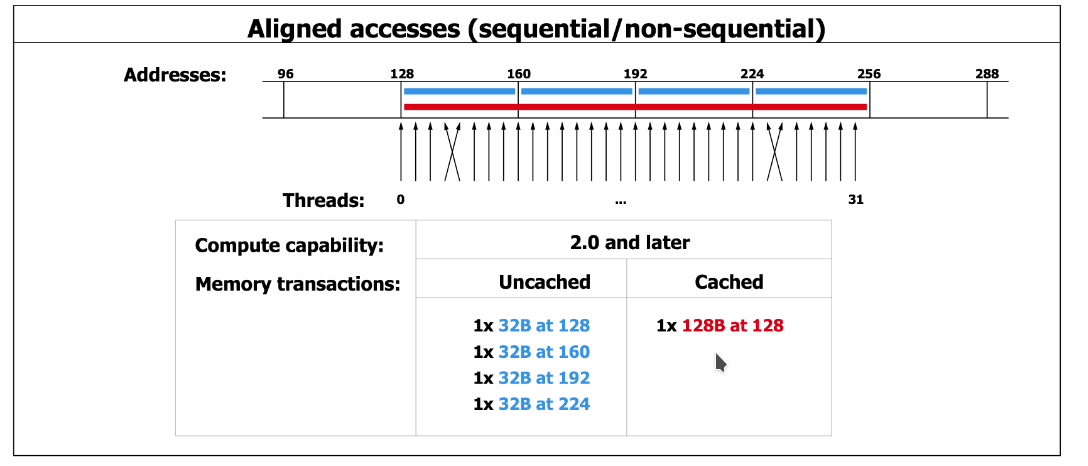
\includegraphics[scale=0.35]{images/coalesced_memory_aligned.png} %[3h]
\end{center}
\end{figure}

\end{frame}

\begin{frame}[t]{What is coalesced memory access?}
If threads in a warp access nearby memory locations then these memory requests can be \textbf{coalesced} into fewer transactions\cite{nv_prog_guide}. 

\bigskip 

\begin{figure}
\begin{center}
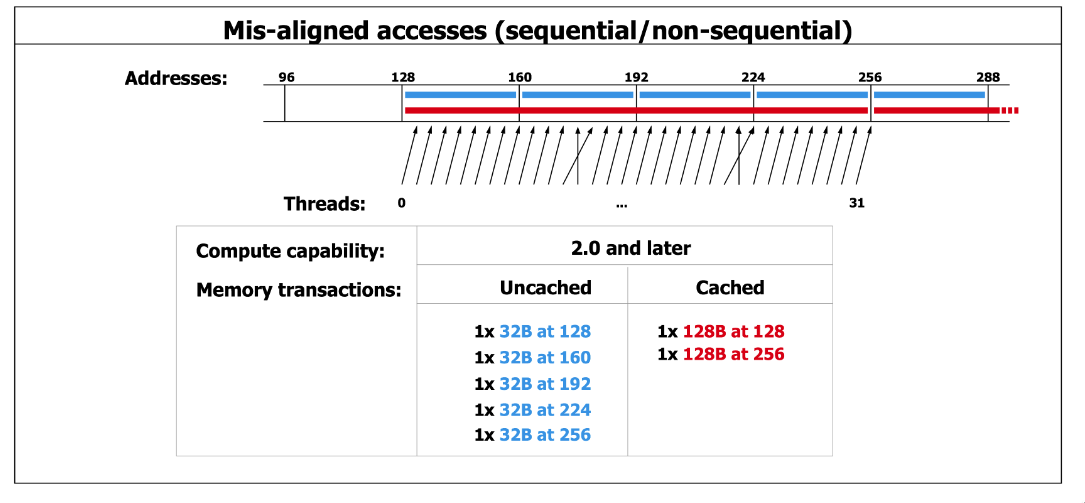
\includegraphics[scale=0.35]{images/coalesced_memory_unaligned.png} %[3h]
%[3h]
\end{center}
\end{figure}

\end{frame}

\begin{frame}{Coalesced Memory: CPUs vs GPUs}
\textbf{CPU} approach: \emphasize{Array of Structures}
\begin{center}
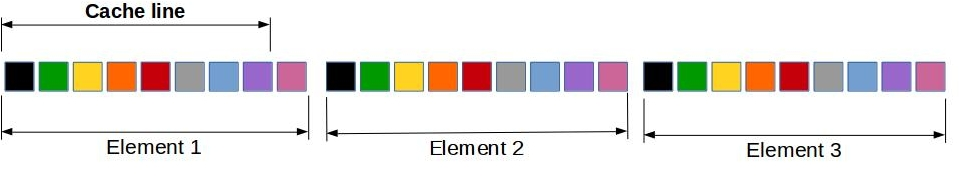
\includegraphics[scale=0.3]{images/coalesced-memory-access-2.jpg} %[3h]
%[3h]
\end{center}

\textbf{GPU} approach: \emphasize{Structure of Arrays}
\begin{center}
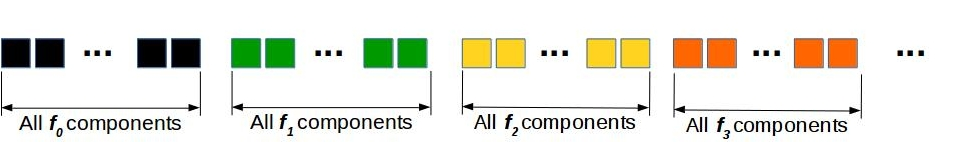
\includegraphics[scale=0.3]{images/coalesced-memory-access-1.jpg} %[3h]
%[3h]
\end{center}
\end{frame}
%%%%%%%%%%%%%%%%%%%%%%%%%%%%%%%%%%%%%%%%%%%%%%%%%%%%%%%%%%%%%%%%
%------------------------- CUDA Restrictions
\begin{frame}[t]{CUDA Execution Parameters}
%[4h]
\textbf{Hardware limits} on the number of threads and blocks: 

\bigskip

\begin{center}

\begin{tabular}{|c|c|c|c|}
\hline
Compute Capability & 2.0 & 3.0 & 5.0 \\
\hline
Max. blocks & 65535 & $2^{31}-1$ & $2^{31}-1$ \\
\hline
Max. threads per block & 1024 & 1024 & 1024 \\
\hline
Warp size & 32 & 32 & 32 \\ 
\hline
Resident blocks per MP & 8 & 16 & 32 \\ 
\hline
Resident threads per MP & 1536 & 2048 & 2048 \\
\hline
Resident warps per MP & 48 & 64 & 64 \\ 
\hline

\end{tabular}
\end{center}

\end{frame}

\begin{frame}[t]{CUDA Execution Parameters}
%[4h]
There is a similar \textbf{limit} on the number of registers: 

\bigskip

\begin{center}

\begin{tabular}{|c|c|c|c|}
\hline
Compute Capability & 2.0 & 3.0 & 5.0 \\
\hline
Number of registers per MP & 32 K & 64 K & 64 K \\
\hline
Max. registers per block & 32 K & 64 K & 64 K  \\
\hline
Max. registers per thread & 63 & 255 & 255 \\ 
\hline

\end{tabular}
\end{center}

\bigskip

Why are these important? 

\pause 

\bigskip

They all affect \textbf{occupancy}. 

\end{frame}

%------------------- Occupancy Calculation --------------

\begin{frame}[t]{Occupancy}

\[ Occupancy = \frac{\text{Active warps per multiprocessor} } {\text {Max. resident warps per multiprocessor} } \]

\pause 

\begin{itemize}
	\medskip
	\item Low occupancy means that you cannot hide memory latency by switching between different warps. 
    
    \pause
    \medskip
    \item On the other hand, high occupancy can lead to register spillage and thereby decrease performance. 
    
    \pause
    \medskip
    \item Therefore, we need to balance at least two things: 
    \medskip
    \begin{enumerate}
    	\item Choose grid and block size such that we can maximize multiprocessor usage. 
        \pause 
        \smallskip
        \item At the same, ensure that registers used per thread are low enough to fit everything in the register file.  
    \end{enumerate}
\end{itemize}

\end{frame}

%-----------------------Occupancy Example ----------------------

\begin{frame}[t]{Occupancy Example: Threads and Blocks}
Compute capability 2.0: 1536 threads and 8 blocks per multiprocessor.

\[ \text{Total threads per MP} = \text{Blocks per MP} \times \text{Threads per block} 
\]
\begin{itemize}
	\item For a kernel with 32 threads per block, we need 1536 / 32 = 48 blocks to fully occupy the MP. However, devices with compute capability 2.0 \emphasize{only support 8 blocks/MP.}
    
    \pause 
    \medskip
    
    \item To fully occupy such a GPU, we need to launch kernels with 1536 / 8 = 192  threads per block. 
    
    \pause 
    \medskip
    
    \item This gives 6 warps per block and a total of $ 6 \times 8 = 48 $ warps / MP. This is the maximum number of active warps per MP for such a device.
    
\end{itemize}
\end{frame}

%Occupancy Registers

\begin{frame}{Occupancy Example: Registers}
Devices with compute capability 2.0 have \emphasize{32,768} registers per multiprocessor. Continuing with the example, suppose we have a kernel that uses 21 registers per thread. 

\pause

\begin {itemize}
	\medskip
	\item With 1536 threads per MP, our register usage is 1536 * 21 = \emphasize{32,256}. In this case we are fine.  
    
    \pause 
    \medskip
    
    \item Now assume register usage per kernel is 22. Then to run 1536 threads, we would need 1536 * 22 = \emphasize{33,972} registers. This will lead to \emphasize{register spilling}. 
    
    \pause
    \medskip
    \item Here reducing the occupancy by reducing the number of threads might speed up the application: 32768 / 22 = \emphasize{1489 max. threads} without register spilling. We can only have 7 active blocks with 192 threads per block and a \emphasize{total of 1344 threads}. 
    
\end{itemize}
\end{frame}

%Register Usage Data
\begin{frame}{Getting register usage data}

Use the compiler flag \texttt{-Xptxas -v} to get register usage per kernel. 

\begin{figure}
\begin{center}
	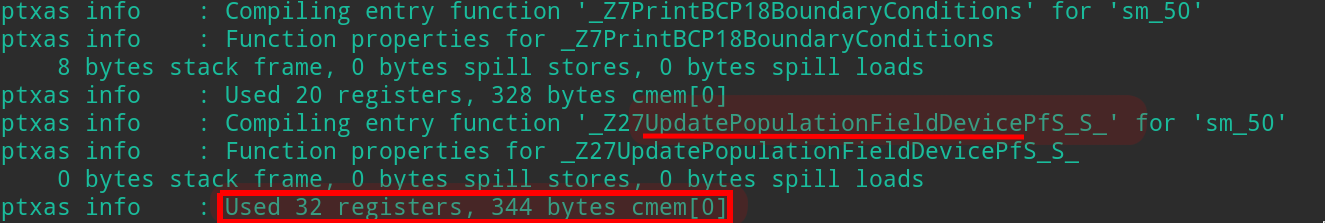
\includegraphics[scale=0.30]{images/register_usage_highlighted.png}
\end{center}
\end{figure}
\end{frame}


%--------------------- Occupancy Calculator ------------------

\begin{frame}[t]{NVIDIA Occupancy Calculator}
In order to figure out the right block and thread distribution for a given number of registers per thread, you can use NVIDIA's occupancy calculator. 

\begin{figure}
\begin{center}
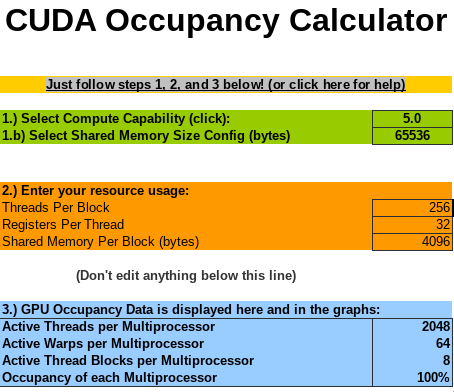
\includegraphics[scale=0.5]{images/cuda_occupancy_calc.png}<1>
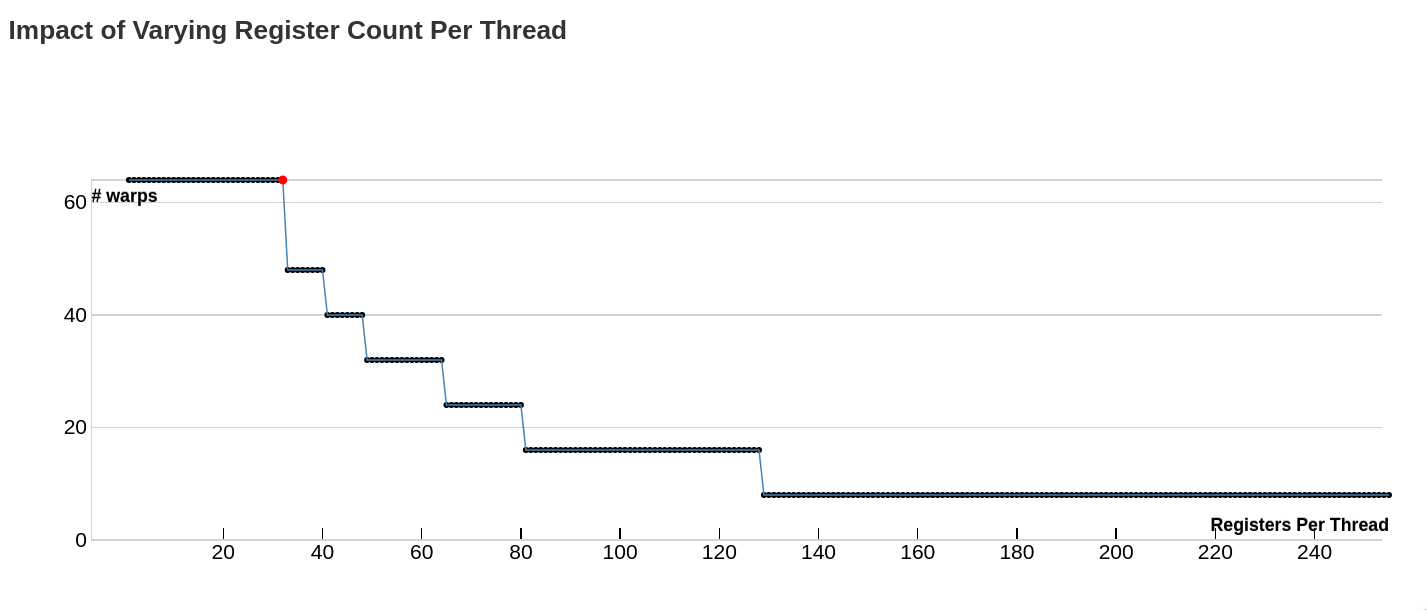
\includegraphics[scale=0.3]{images/cuda_occupancy_registers.png}<2>
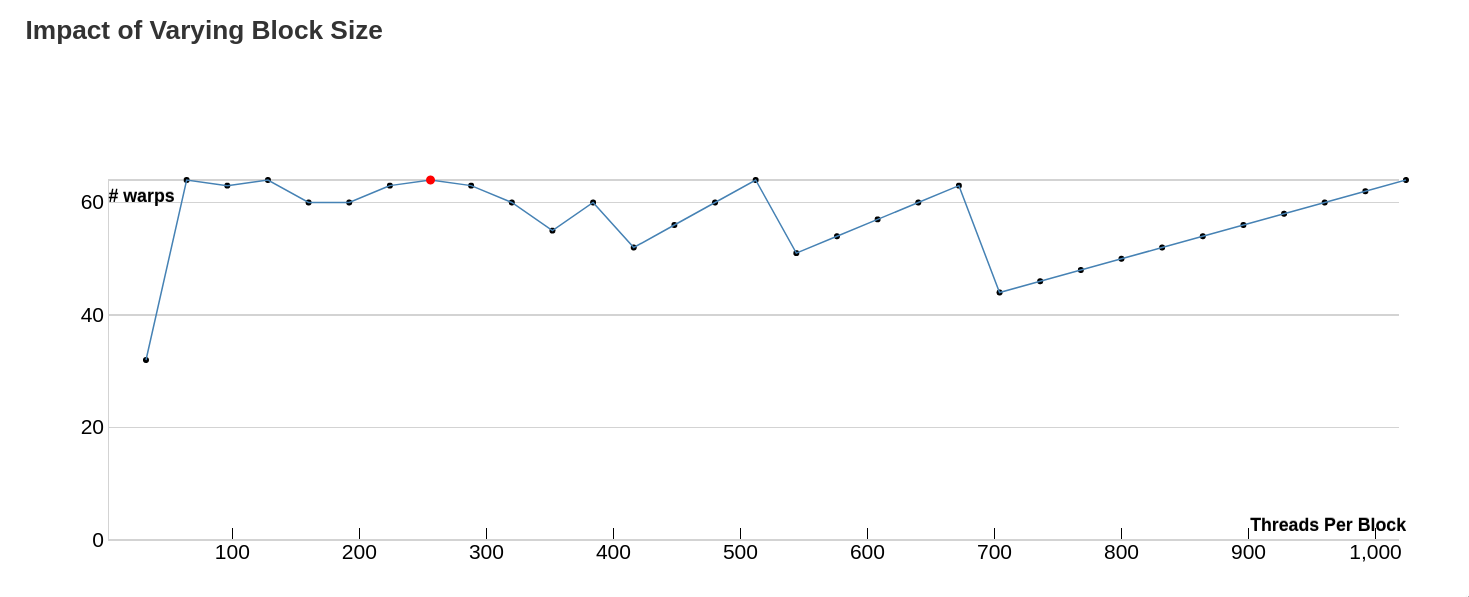
\includegraphics[scale=0.3]{images/cuda_occupancy_threads.png}<3>

\end{center}
\end{figure}
\end{frame}

%-------------------- Visual Profiler------------------------

\begin{frame}{Nvidia Visual Profiler}
You can use Nvidia's Visual Profiler to find the achieved occupancy. 

\begin{figure}
\begin{center}
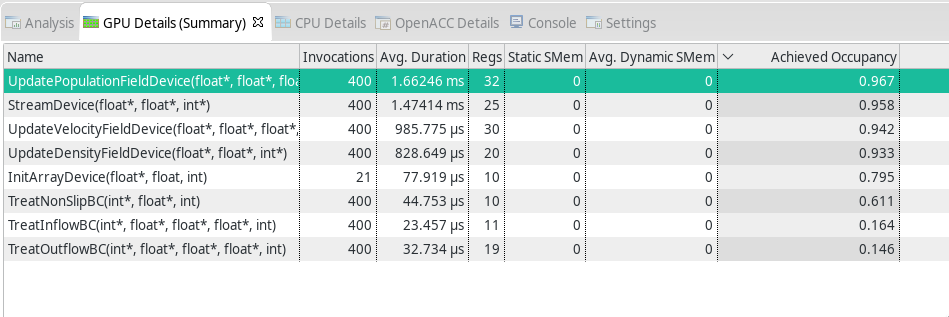
\includegraphics[scale=0.4]{images/nvvp_profile.png}
\end{center}
\end{figure}

\end{frame}

%%%%%%%%%%%%%%%%%%%%%%%%%%%%%%%%%%%%%%%%%%%%%%%%%%%%%%
%Branch Divergence: 1
\section{Branch divergence within a warp}
\begin{frame}[t]{Branch Divergence }
\begin{itemize}
\item You have probably already heard about \textbf{branch divergence within a warp}.
\item You might also have seen this figure: \\
\end{itemize}
\end{frame}

%Branch Divergence: 2
\begin{frame}[t]{Branch Divergence }
\begin{itemize}
\item You have probably already heard about \textbf{branch divergence within a warp}.
\item You might also have seen this figure: \\
\end{itemize}
\begin{figure}
	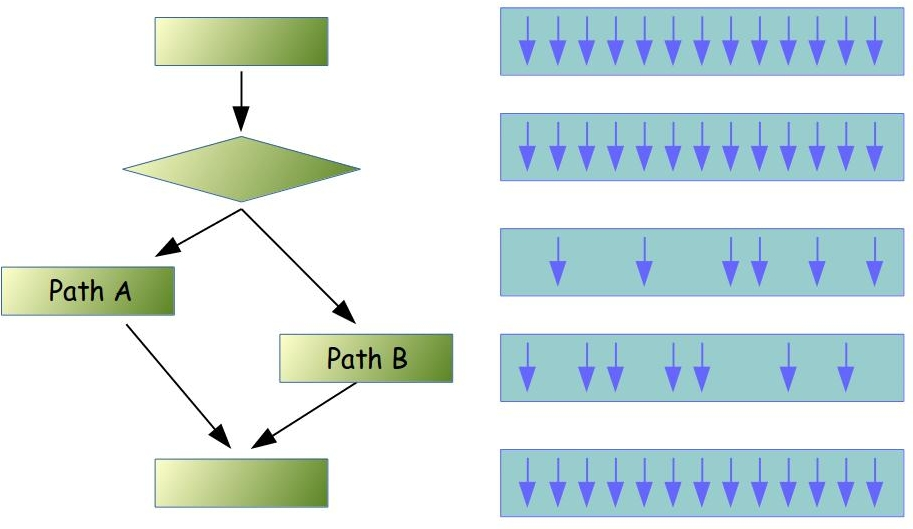
\includegraphics[scale=0.22]{images/bd-1.jpg}
	\centering
\end{figure}
\end{frame}

%Branch Divergence: 3
\begin{frame}[t]{Branch Divergence }
\begin{itemize}
\item You have probably already heard about \textbf{branch divergence within a warp}.
\item You might also have seen this figure: \\
\end{itemize}
\begin{figure}
	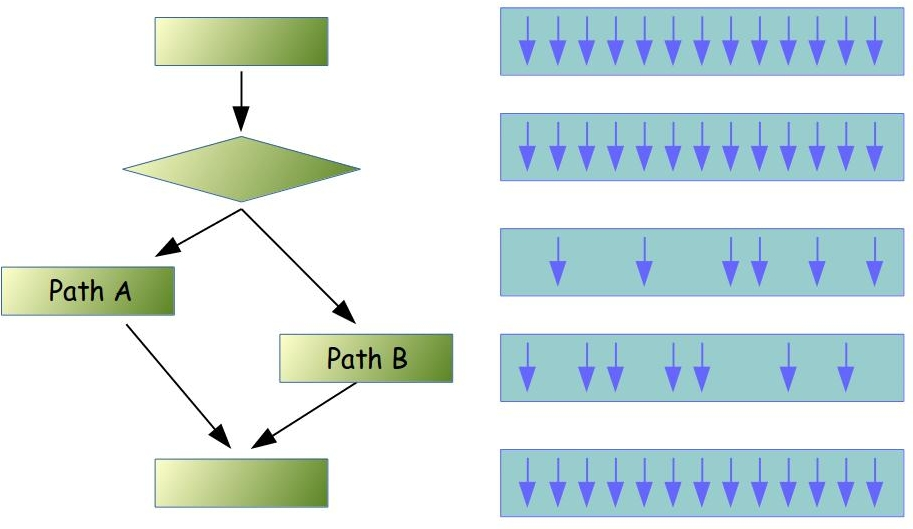
\includegraphics[scale=0.22]{images/bd-1.jpg}
	\centering
\end{figure}
\begin{itemize}
\item You know that branches are executed in <<lockstep>>
\end{itemize}
\end{frame}

%Branch Divergence: 4
\begin{frame}[t]{Branch Divergence }
\begin{itemize}
\item You have probably already heard about \textbf{branch divergence within a warp}.
\item You might also have seen this figure: \\
\end{itemize}
\begin{figure}
	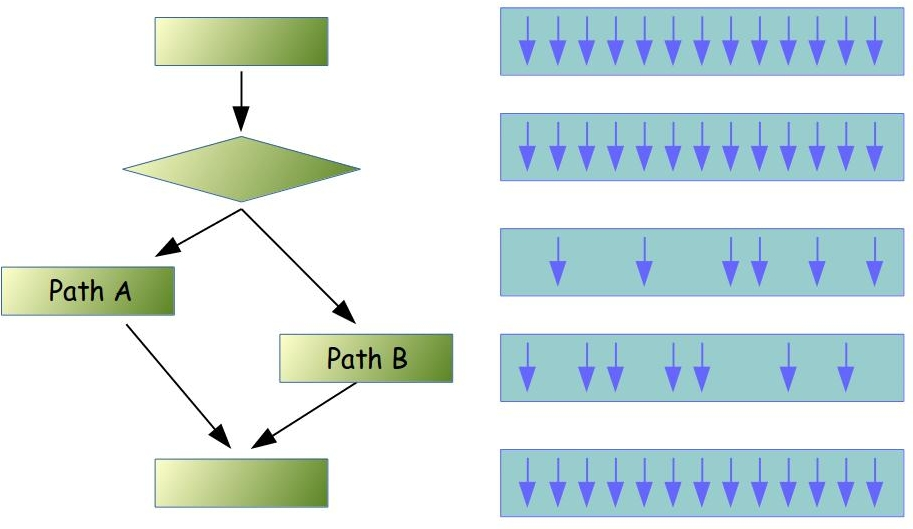
\includegraphics[scale=0.22]{images/bd-1.jpg}
	\centering
\end{figure}
\begin{itemize}
\item You know that branches are executed in <<lockstep>>
\item You might already know that this leads to almost \emphasize{50\% performance loss}

\end{itemize}
\end{frame}


%Branch Divergence: 5
\begin{frame}[t]{Branch Divergence }
\begin{itemize}
\item You have probably already heard about \textbf{branch divergence within a warp}.
\item You might also have seen this figure: \\
\end{itemize}
\begin{figure}
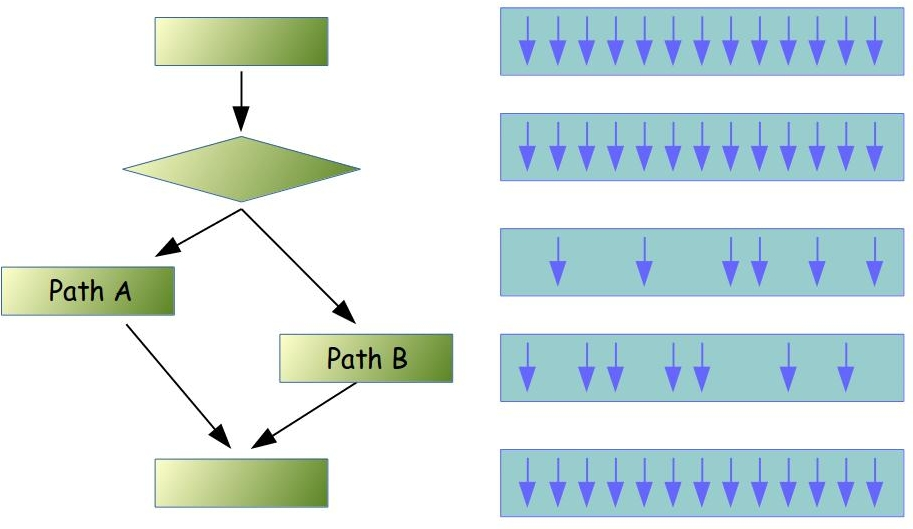
\includegraphics[scale=0.22]{images/bd-1.jpg}
\centering
\end{figure}
\begin{itemize}
\item You know that branches are executed in <<lockstep>>
\item You might already know that this leads to almost \emphasize{50\% performance loss}
\item Question: is this \textbf{always} true?
\end{itemize}
\end{frame}


%Branch Divergence: 6
\begin{frame}[t]{Branch Divergence }
What \textbf{assumptions} did we make to get a \emphasize{50\% performance loss}?
\end{frame}

%Branch Divergence: 7
\begin{frame}[t]{Branch Divergence }
What \textbf{assumptions} did we make to get a \emphasize{50\% performance loss}?
\begin{itemize}
\item One \textbf{half} of the warp executes \textbf{Branch A} and the second half executes \\ \textbf{Branch B}
\end{itemize}
\end{frame}

%Branch Divergence: 8
\begin{frame}[t]{Branch Divergence }
What \textbf{assumptions} did we make to get a \emphasize{50\% performance loss}?
\begin{itemize}
	\item One \textbf{half} of the warp executes \textbf{Branch A} and the second half executes \\ \textbf{Branch B}.
\item The \textbf{workloads} are \textbf{equal}.
\end{itemize}
\end{frame}


%Branch Divergence: 9
\begin{frame}[t]{Branch Divergence }
What \textbf{assumptions} did we make to get a \emphasize{50\% performance loss}?
\begin{itemize}
	\item One \textbf{half} of the warp executes \textbf{Branch A} and the second half executes \\ \textbf{Branch B}.
	\item The \textbf{workloads} are \textbf{equal}.
\end{itemize}

\begin{alertblock}{Extreme case}
\begin{itemize}
\item Consider \textbf{32} distinct \textbf{branches}.
\item Each \textbf{thread} executes \textbf{one branch}.
\item All branches have \textbf{the same workload}.
\item The \textbf{slow-down} is \textbf{x32} in that case.
\end{itemize}

\end{alertblock}
\end{frame}


%Branch Divergence: 10
\begin{frame}[t]{Branch Divergence }
What \textbf{assumptions} did we make to get a \emphasize{50\% performance loss}?
\begin{itemize}
	\item One \textbf{half} of the warp executes \textbf{Branch A} and the second half executes \\ \textbf{Branch B}.
	\item The \textbf{workloads} are \textbf{equal}.
\end{itemize}

\begin{alertblock}{Extreme case}
	\begin{itemize}
		\item Consider \textbf{32} distinct \textbf{branches}.
		\item Each \textbf{thread} executes \textbf{one branch}.
		\item All branches have \textbf{the same workload}.
		\item The \textbf{slow-down} is \textbf{x32} in that case.
	\end{itemize}
	
\end{alertblock}
\bigskip
\textbf{But} let us consider our case one more time
\end{frame}

%Branch Divergence: 12
\begin{frame}[fragile, t]{Branch Divergence }
Let's compare two implementation of the same algorithm: \textbf{with} branching
\begin{scriptsize}
\begin{lstlisting}
__global__ void UpdateVelocityFieldDevice(real *velocity,
                                          real *population,
                                          real *density,
                                          int *flag_field) {
    int num_lattices = parameters_device.num_lattices;
    short int num_directions = parameters_device.discretization; 
    
    int thread_id = threadIdx.x + blockIdx.x * blockDim.x;
    
    while (thread_id < num_lattices) {
        if (flag_field[thread_id] == FLUID) { // <= branching
            real lattice_velocity_x = 0.0;
            real lattice_velocity_y = 0.0;
            
            for (short int component = 0; component < num_directions; ++component) {
                real distribution = population[component * num_lattices + thread_id];
                lattice_velocity_x += coords_device[component] * distribution;
                lattice_velocity_y += coords_device[num_directions + component] * distribution;
            }

            real inverse_density = 1.0 / density[thread_id];
            velocity[thread_id] = inverse_density * lattice_velocity_x;
            velocity[num_lattices + thread_id] = inverse_density * lattice_velocity_y;
        }
        thread_id += blockDim.x * gridDim.x; 
    }
}

\\ MLUPS: 42.79 | 19.98  [float | double] (GeForce 610M)
\end{lstlisting}
\end{scriptsize}
\end{frame}


%Branch Divergence: 13
\begin{frame}[fragile, t]{Branch Divergence }
Let's compare two implementation of the same algorithm: \textbf{without} branching
\begin{scriptsize}
\begin{lstlisting}
__global__ void UpdateVelocityFieldDevice_A(real *velocity,
                                            real *population,
                                            real *density,
                                            int *flag_field,
                                            int *fluid_indices, // additional parameter
                                            int num_fluid_lattices) {
    int num_lattices = parameters_device.num_lattices;
    short int num_directions = parameters_device.discretization; 
    
    int thread_id = threadIdx.x + blockIdx.x * blockDim.x;
    while (thread_id < num_fluid_lattices) {
        int index = fluid_indices[thread_id]; // <-----
        
        real lattice_velocity_x = 0.0;
        real lattice_velocity_y = 0.0;
            
        for (short int component = 0; component < num_directions; ++component) {
            real distribution = population[component * num_lattices + index];
            lattice_velocity_x += coords_device[component] * distribution;
            lattice_velocity_y += coords_device[num_directions + component] * distribution;
        }

        real inverse_density = 1.0 / density[index];
        velocity[index] = inverse_density * lattice_velocity_x;
        velocity[num_lattices + index] = inverse_density * lattice_velocity_y;
        
        thread_id += blockDim.x * gridDim.x; 
    }
}

\\ MLUPS: ??.?? | ??.??  [float | double] (GeForce 610M)
\end{lstlisting}
\end{scriptsize}
\end{frame}


%Branch Divergence: 13
\begin{frame}[fragile, t]{Branch Divergence }
Let's compare two implementations of the same algorithm: \textbf{without branching} 
\begin{scriptsize}
\begin{lstlisting}
__global__ void UpdateVelocityFieldDevice_A(real *velocity,
                                            real *population,
                                            real *density,
                                            int *flag_field,
                                            int *fluid_indices, // additional parameter
                                            int num_fluid_lattices) {
    int num_lattices = parameters_device.num_lattices;
    short int num_directions = parameters_device.discretization; 
    
    int thread_id = threadIdx.x + blockIdx.x * blockDim.x;
    while (thread_id < num_fluid_lattices) {
        int index = fluid_indices[thread_id]; // it leads to indirect addressing
        
        real lattice_velocity_x = 0.0;
        real lattice_velocity_y = 0.0;
            
        for (short int component = 0; component < num_directions; ++component) {
            real distribution = population[component * num_lattices + index];
            lattice_velocity_x += coords_device[component] * distribution;
            lattice_velocity_y += coords_device[num_directions + component] * distribution;
        }

        real inverse_density = 1.0 / density[index];
        velocity[index] = inverse_density * lattice_velocity_x;
        velocity[num_lattices + index] = inverse_density * lattice_velocity_y;
        
        thread_id += blockDim.x * gridDim.x; 
    }
}

\\ MLUPS: 42.22 | 18.44  [float | double] (GeForce 610M)
\end{lstlisting}
\end{scriptsize}
\end{frame}

%Branch Divergence: 11
\begin{frame}[t]{Branch Divergence }
\begin{figure}
	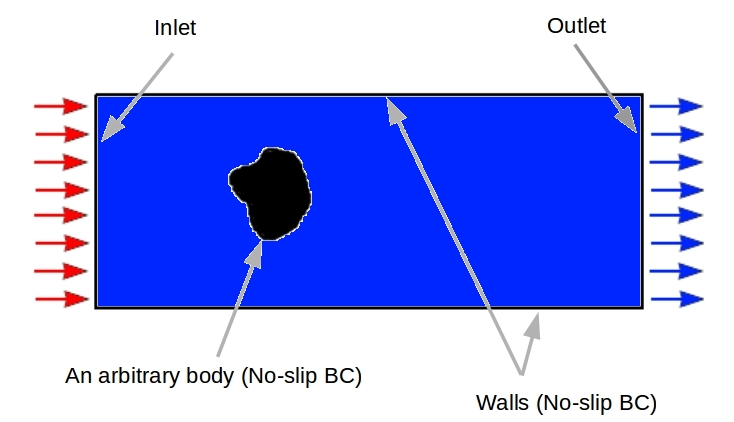
\includegraphics[scale=0.3]{images/wind-tunnel-1.jpg}
	\centering
\end{figure}

\begin{itemize}
\item Almost \textbf{95\%} of cells are fluid cells whereas there are only approximately \textbf{5\%} boundary cells.

\item The work load is \textbf{significantly} different during the \textbf{Collision} step.
	\begin{itemize}
	\item For a \textbf{<<FLUID>>} cell, update \textbf{density, velocity, distribution}.
	\item \textbf{Do nothing} for a \textbf{BC}. 
	\end{itemize}
\end{itemize}
\end{frame}

\begin{frame}[t]{Branch Divergence}
\begin{itemize}
\item We have just seen an example where a branching code \textbf{outperforms} a non-branching code. 

\item In this case, branch divergence helps preserve the key property of the algorithm: \textbf{structured mesh} (direct memory addressing).

\item The implementation without branching is, in its turn, a \textbf{linked list}: the address of the next element must be fetched from the memory.

\item Moreover, it needs \textbf{additional memory transfers} (expensive)
\end{itemize}

\textbf{Question:} What about the \emphasize{Porous Media case}? Is that also true for that scenario? 
\\~\\
Let's take a look...
\end{frame}

\begin{frame}[t]{Branch Divergence: Porous Media case}
\begin{figure}
	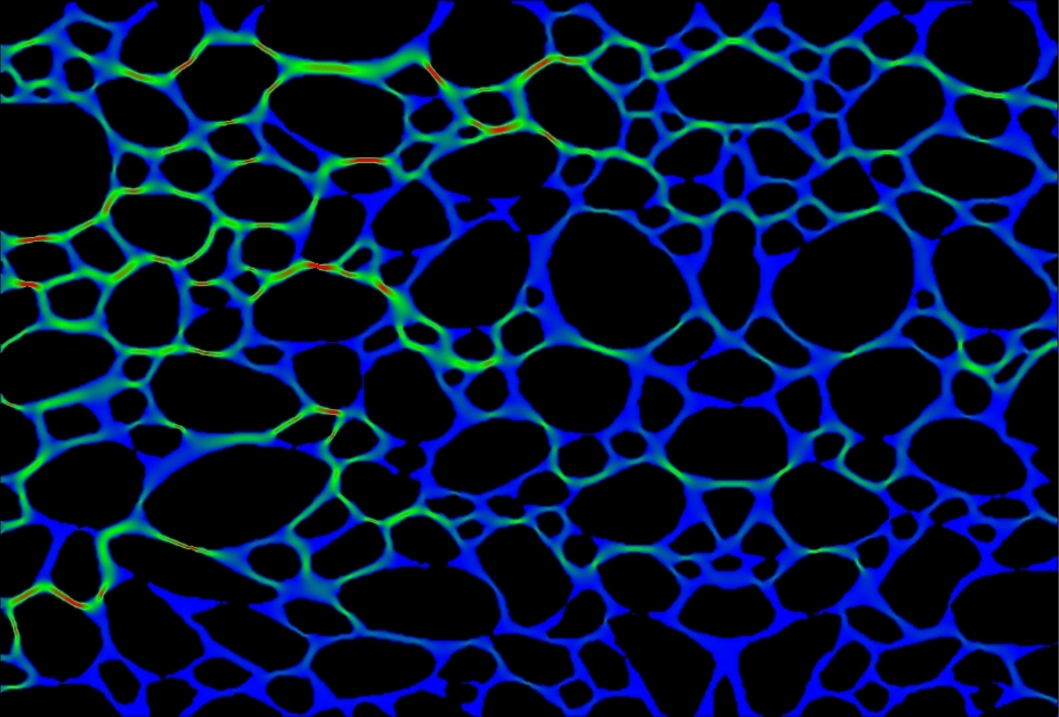
\includegraphics[scale=0.18]{images/porous-media-case.jpg}
	\centering
\end{figure}
MLUPS (with branching): 46.21 | 26.55 [float | double] (Geforce 610M)

MLUPS (without branching): ??.?? | ??.?? [float | double] (Geforce 610M)

\end{frame}

\begin{frame}[t]{Branch Divergence: Porous Media case}
\begin{figure}
	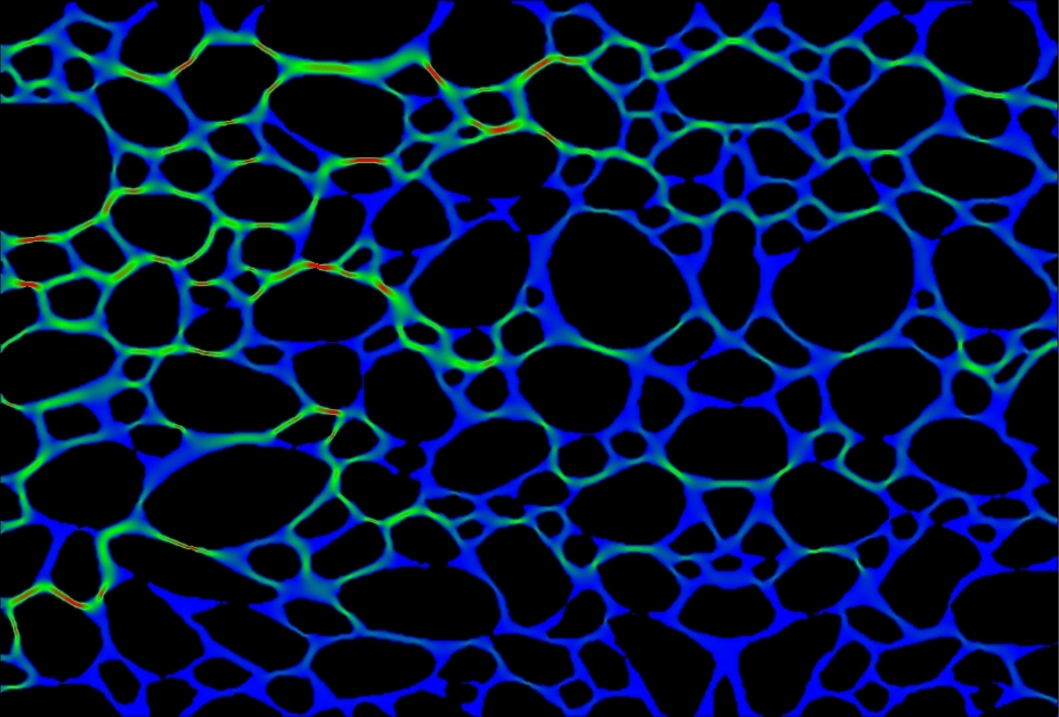
\includegraphics[scale=0.18]{images/porous-media-case.jpg}
	\centering
\end{figure}
MLUPS (with branching): 46.21 | 26.55 [float | double] (Geforce 610M)\\

MLUPS (without branching): \emphasize{49.85 | 28.02} [float | double] (Geforce 610M)
\end{frame}

\begin{frame}[t]{Branch Divergence: Porous Media case}
\begin{figure}
	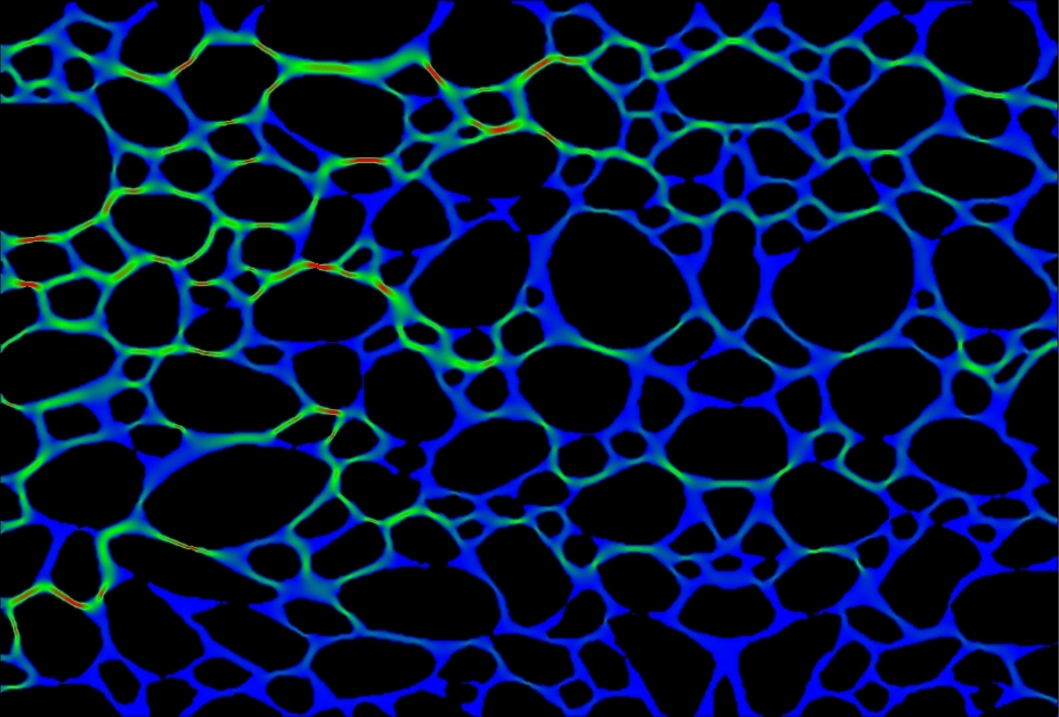
\includegraphics[scale=0.18]{images/porous-media-case.jpg}
	\centering
\end{figure}
MLUPS (with branching): 46.21 | 26.55 [float | double] (Geforce 610M)\\

MLUPS (without branching): \emphasize{49.85 | 28.02} [float | double] (Geforce 610M)

\begin{alertblock}{Note}
The right decision heavily depends on your specific scenario
\end{alertblock}
\end{frame}

\begin{frame}[t]{Branch Divergence}
\begin{itemize}
\item We have just seen an example where a branching code \textbf{outperforms} a non-branching code. 

\item In this case, branch divergence helps preserve the key property of the algorithm: \textbf{structured mesh} (direct memory addressing).

\item The implementation without branching is, in its turn, a \textbf{linked list}: the address of the next element must be fetched from the memory.

\item Moreover, it needs \textbf{additional memory transfers} (expensive)

\item \emphasize{But} sometimes it is \textbf{better to get rid of branching}.

\end{itemize}

\textbf{Question:} What about Boundary Elements? Can we still use branching?
\\~\\
Let's look at the computational scheme one more time...
\end{frame}


%Branch Divergence: 14
\begin{frame}[t]{Branch Divergence: Boundary Conditions}
\begin{figure}
	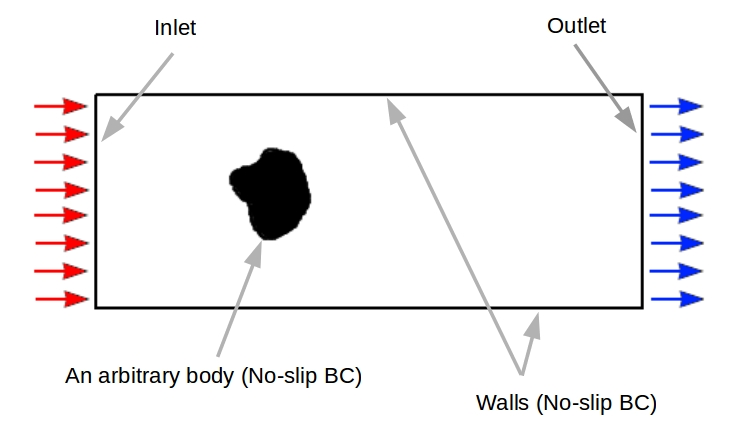
\includegraphics[scale=0.3]{images/wind-tunnel.jpg}
	\centering
\end{figure}

\begin{itemize}
\item Almost \textbf{5\%} of cells are boundary cells. The rest are fluid cells.

\item The workload is \textbf{significantly} different during \textbf{Boundary Update} step.
\medskip
	\begin{itemize}
	\item For \textbf{<<FLUID>>}, \textbf{do nothing}
	\item For a \textbf{boundary cell}, \textbf{update} corresponding boundary.
	\end{itemize}
\end{itemize}
\end{frame}


\begin{frame}[t]{Branch Divergence: Boundary Conditions}
\begin{itemize}
\item For boundary cells, \textbf{branching} can lead to \textbf{wastage of resources}.
\medskip
\item Most \textbf{cores are usually idle} and are probably \textbf{waiting for a thread} in their warp.
\medskip
\item It is much better to \textbf{update boundary elements separately} from <<FLUID>> elements.
\smallskip
\item Additionally it is better to update each boundary condition separately.
\medskip
\item This approach brings us \textbf{functional parallelism}
\medskip
\item This is a great opportunity to try out \textbf{asynchronous kernel launch} and execution. 
\end{itemize}
\end{frame}



%%%%%%%%%%%%%%%%%%%%%%%%%%%%%%%%%%%%%%%%%%%%%%%%%%%%%%
% Asynchronous kernel launch : 1
\section{Asynchronous kernel launch}
\begin{frame}{Synchronicity in Cuda}
\begin{itemize}
\item CUDA calls can be either \textbf{synchronous} or \textbf{asynchronous} with respect to
the host
\begin{itemize}
\item \emphasize{Synchronous:} submit work and wait for completion
\smallskip
\item \emphasize{Asynchronous:} submit work and return immediately
\end{itemize}
\medskip
\item Kernel launches are non-blocking and automatically overlap with the
host
\end{itemize}

\begin{figure}
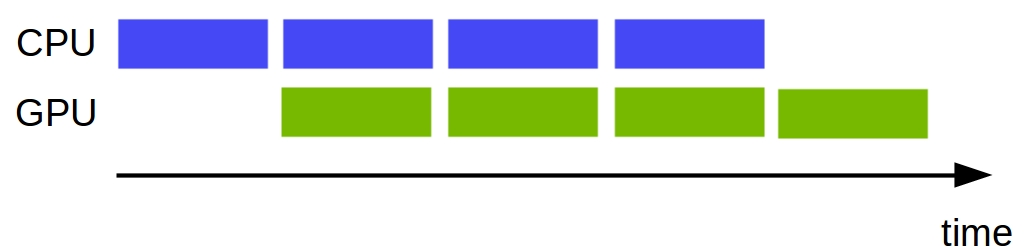
\includegraphics[scale=0.25]{images/ans-kernel-exe-1.jpg}
\centering
\end{figure}
\end{frame}


% Asynchronous kernel launch : 2
\begin{frame}[t]{Cuda Streams}
\begin{itemize}
\item A stream is a \textbf{queue} of device work
	\begin{itemize}
	\item The host places work in the queue and continues on immediately
	\item Device schedules work from streams when resources are free
	\end{itemize}

\item All CUDA operations are placed within a stream

\item Operations within the \emphasize{same stream} are \emphasize{ordered} \textbf{(FIFO)} and
cannot overlap

\item Operations in \emphasize{different streams} are \emphasize{unordered} and can
overlap

\end{itemize}
\end{frame}

% Asynchronous kernel launch : 3
\begin{frame}[t]{Managing Streams}
\begin{itemize}
\item Declares a stream handle: \textit{cudaStream\_t stream;}
\medskip
\item Allocates a stream: \textit{cudaStreamCreate(\&stream);}
\medskip
\item Deallocates a stream: \textit{cudaStreamDestroy(stream);}
\medskip
\end{itemize}
\end{frame}

% Asynchronous kernel launch : 4
\begin{frame}[t]{Managing Streams}
\begin{itemize}
\item Declares a stream handle: \textit{cudaStream\_t stream;}
\medskip
\item Allocates a stream: \textit{cudaStreamCreate(\&stream);}
\medskip
\item Deallocates a stream: \textit{cudaStreamDestroy(stream);}
\medskip
\end{itemize}

\textbf{Question}: How to assign work to a stream?
\end{frame}


% Asynchronous kernel launch : 5
\begin{frame}[t]{Managing Streams}
\begin{itemize}
\item Declares a stream handle: \textit{cudaStream\_t stream;}
\medskip
\item Allocates a stream: \textit{cudaStreamCreate(\&stream);}
\medskip
\item Deallocates a stream: \textit{cudaStreamDestroy(stream);}
\medskip
\end{itemize}

\textbf{Question}: How to assign work to a stream?
 
\begin{itemize}
\item Stream is the 4th launch parameter\\
\[kernel \lll blocks , threads, smem, stream \ggg (); \]
\\~\\
\item Streams are passed to some API calls\\
\[cudaMemcpyAsync( dst, src, size, dir, stream); \]
\end{itemize}
\end{frame}


% Asynchronous kernel launch : 6
\begin{frame}[t]{Default Stream}
\begin{itemize}
\item If no stream is specified explicitly, a call will be assigned to \textbf{the default stream}: \emphasize{Stream 0}
\end{itemize}
\end{frame}

% Asynchronous kernel launch : 7
\begin{frame}[t]{Default Stream}
\begin{itemize}
\item If no stream is specified explicitly, a call will be assigned to \textbf{the default stream}: \emphasize{Stream 0}

\item Stream 0 has its own special synchronization rule:
\begin{alertblock}{Rule}
Operations in stream 0 cannot overlap other streams\\
In other words, the hardware will wait untill all other streams finish their work before scheduling \textbf{stream 0}
\end{alertblock}
\end{itemize}
\end{frame}

% Asynchronous kernel launch : 8
\begin{frame}[t]{Default Stream}
\begin{itemize}
\item If no stream is specified explicitly, a call will be assigned to \textbf{the default stream}: \emphasize{Stream 0}

\item Stream 0 has its own special synchronization rule:
\begin{alertblock}{Rule}
Operations in stream 0 cannot overlap with other streams.\\
In other words, the hardware will wait untill all other streams finish their work before scheduling \textbf{stream 0}.
\end{alertblock}
\end{itemize}

\begin{figure}
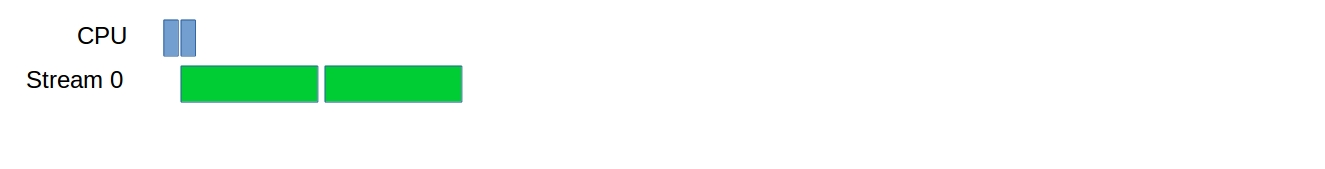
\includegraphics[scale=0.25]{images/ans-kernel-launch-1.jpg}
\centering
\end{figure}

\end{frame}


% Asynchronous kernel launch : 9
\begin{frame}[t]{Default Stream}
\begin{itemize}
\item If no stream is specified explicitly, a call will be assigned to \textbf{the default stream}: \emphasize{Stream 0}

\item Stream 0 has its special synchronization rule:
\begin{alertblock}{Rule}
Operations in stream 0 cannot overlap with other streams.\\
In other words, the hardware will wait untill all other streams finish their work before scheduling \textbf{stream 0}.
\end{alertblock}
\end{itemize}

\begin{figure}
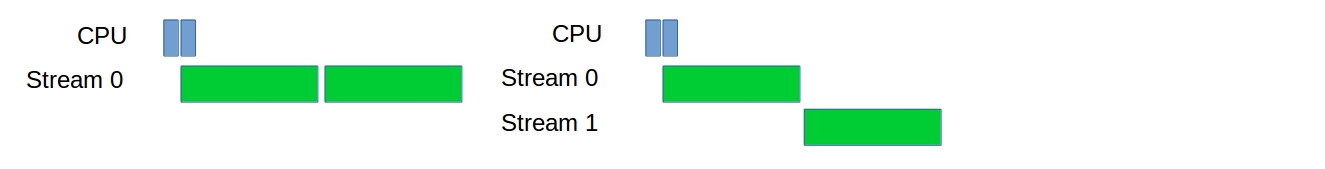
\includegraphics[scale=0.25]{images/ans-kernel-launch-2.jpg}
\centering
\end{figure}

\end{frame}


% Asynchronous kernel launch : 10
\begin{frame}[t]{Default Stream}
\begin{itemize}
\item If no stream is specified explicitly, a call will be assigned to \textbf{the default stream}: \emphasize{Stream 0}

\item Stream 0 has its own special synchronization rule:
\begin{alertblock}{Rule}
Operations in stream 0 cannot overlap with other streams.\\
In other words, the hardware will wait untill all other streams finish their work before scheduling \textbf{stream 0}.
\end{alertblock}
\end{itemize}

\begin{figure}
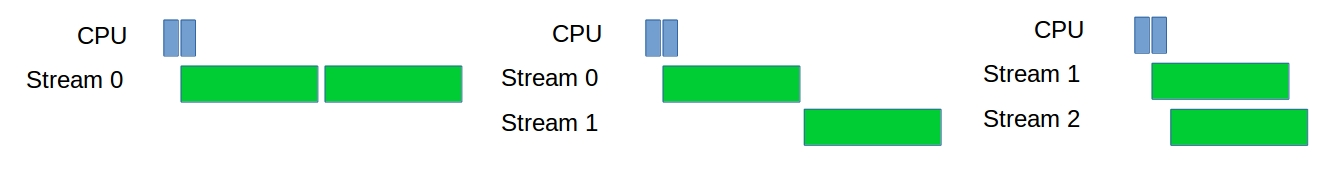
\includegraphics[scale=0.25]{images/ans-kernel-launch-3.jpg}
\centering
\end{figure}

\end{frame}


% Asynchronous kernel launch : 11
\begin{frame}[t]{Strategies}
\textbf{Question:} When to use asynchronous CUDA calls?

\begin{itemize}
\item When your kernels \textbf{cannot} occupy the entire device (all Streaming Multiprocessors)\\
\emphasize{Attention:} you need \textbf{function parallelism} for that
\\~\\
\item When you can overlay kernel execution with data transfer between the host and device memory
\end{itemize}

\medskip
Example: update of \textbf{Boundary Conditions}
\begin{figure}
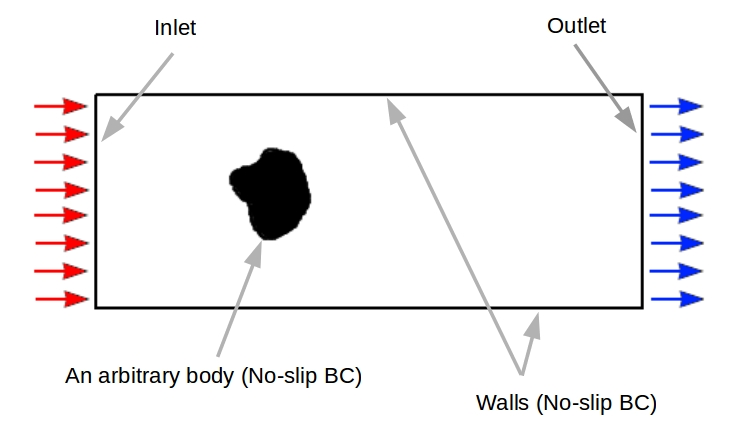
\includegraphics[scale=0.27]{images/wind-tunnel.jpg}
\centering
\end{figure}
\end{frame}

% Asynchronous kernel launch : 12
\begin{frame}[t]{Performance gain: data transfer overlap}
Performance can be improved \textbf{significantly} if you can \textbf{overlay data transfer} with kernel execution.
\\~\\
Advice: Try to completely hide communication between host and device\\
\medskip
Use: 
\[cudaMemcpyAsync( dst, src, size, dir, stream); \]
\end{frame}

% Asynchronous kernel launch : 13
\begin{frame}[t]{Performance gain: function parallelism}
In general it is \textbf{quite difficult} to get some decent performance gain using \textbf{functional parallelism}: usually your independent kernels are \textbf{too small}
\end{frame}

% Asynchronous kernel launch : 14
\begin{frame}[t]{Performance gain: function parallelism}
In general it is \textbf{quite difficult} to get decent performance gain using \textbf{functional parallelism}: usually your independent kernels are \textbf{too small}
\begin{figure}
	Before\\
	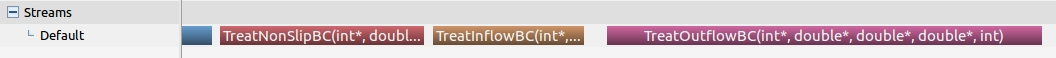
\includegraphics[scale=0.25]{images/streams-1.jpg}
	\centering
\end{figure}
\end{frame}

% Asynchronous kernel launch : 15
\begin{frame}[t]{Performance gain: function parallelism}
In general it is \textbf{quite difficult} to get decent performance gain using \textbf{functional parallelism}: usually your independent kernels are \textbf{too small}
\begin{figure}
	Before\\
	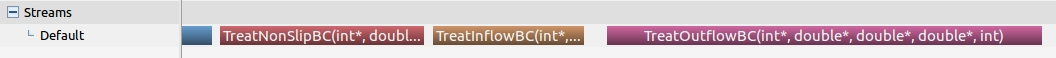
\includegraphics[scale=0.25]{images/streams-1.jpg}
	\centering
\end{figure}

\begin{figure}
	After\\
	\includegraphics[scale=0.25]{images/streams-2.jpg}
	\centering
\end{figure}

\textit{Question:} What performance gain did we get?\\
\end{frame}

% Asynchronous kernel launch : 16
\begin{frame}[t]{Performance gain: function parallelism}
In general it is \textbf{quite difficult} to get decent performance gain using \textbf{functional parallelism}: usually your independent kernels are \textbf{too small}
\begin{figure}
	Before\\
	\includegraphics[scale=0.25]{images/streams-1.jpg}
	\centering
\end{figure}

\begin{figure}
	After\\
	\includegraphics[scale=0.25]{images/streams-2.jpg}
	\centering
\end{figure}

\textit{Question:} What performance gain did we get?\\
\textit{Answer:} \textbf{1.449\%}

\centering{\textbf{Why?}}
\end{frame}

% Asynchronous kernel launch : 17
\begin{frame}[t]{Performance gain: function parallelism}
In general it is \textbf{quite difficult} to get decent performance gain using \textbf{functional parallelism}: usually your independent kernels are \textbf{too small}
\begin{figure}
	Before\\
	\includegraphics[scale=0.25]{images/streams-1.jpg}
	\centering
\end{figure}

\begin{figure}
	After\\
	\includegraphics[scale=0.25]{images/streams-2.jpg}
	\centering
\end{figure}

\textit{Question:} What performance gain did we get?\\
\textit{Answer:} \textbf{1.449\%}

\begin{figure}
	Iteration view
	\includegraphics[scale=0.25]{images/streams-3.jpg}
	\centering
\end{figure}
\end{frame}

% Asynchronous kernel launch : 18
\begin{frame}[t]{Performance gain: function parallelism}
In general it is \textbf{quite difficult} to get some decent performance gain using \textbf{functional parallelism}: usually your independent kernels are \textbf{too small}
\begin{figure}
	Before\\
	\includegraphics[scale=0.25]{images/streams-1.jpg}
	\centering
\end{figure}

\begin{figure}
	After\\
	\includegraphics[scale=0.25]{images/streams-2.jpg}
	\centering
\end{figure}

\textit{Question:} What performance gain did we get?\\
\textit{Answer:} \textbf{1.449\%}

\begin{figure}
	Iteration view
	\includegraphics[scale=0.25]{images/streams-4.jpg}
	\centering
\end{figure}
\end{frame}

%%%%%%%%%%%%%%%%%%%%%%%%%%%%%%%%%%%%%%%%%%%%%%%%%%%%%%%%%%%%%%%%%%%%
%-------------------------OpenGL-------------------------------------

\section{OpenGL}

\begin{frame}{CUDA OpenGL interoperation}

To visualize the results, we use a \textbf{shared buffer} between CUDA and OpenGL. This shared buffer maps the velocity magnitude for each lattice to an RGB value. 

\begin{figure}
\begin{center}
	\includegraphics[scale=0.25]{images/opengl.png}
\end{center}
\end{figure}

\end{frame}

\begin{frame}{Adding Interactivity}
We use GLFW mouse call backs to interactively add obstacles to and remove from the domain. 
\begin{itemize}
	\item Press and drag left mouse button to add obstacles. 
    \item Press and drag right mouse button to erase obstacles. 
\end{itemize}

\pause

\begin{figure}
\begin{center}
	\includegraphics[scale=0.2]{images/mouse_call_backs.png}
\end{center}
\end{figure}
\end{frame}



%-------------------------Bibliography----------------------------
\section{Bibliography}

\begin{frame}[allowframebreaks]

\frametitle{References}
\begin{thebibliography}{10}
	
	\beamertemplateonlinebibitems
	\bibitem{lattice_boltzmann_wiki}
	Lattice Boltzmann Methods (June 8,2018). 
	\newblock Retrieved from https://en.wikipedia.org/wiki/Lattice\_Boltzmann\_methods
	
	
	
	\beamertemplateonlinebibitems
	\bibitem{lattice_boltzmann}
	Lattice Boltzmann Method (June 13,2018). 
	\newblock Retrieved from http://andrew.gibiansky.com/blog/physics/lattice-boltzmann-method/
	
	\beamertemplateonlinebibitems
	\bibitem{lattice_boltzmann_epfl}
	Chen Peng, The Lattice Boltzmann Method for Fluid
	Dynamics: Theory and Applications
	\newblock https://cmcs.epfl.ch/files/content/sites/cmcs/files/People/Peng%20Chen/LBM.pdf


	\beamertemplateonlinebibitems
	\bibitem{nv_prog_guide}
	CUDA C Programming Guide (June 13, 2018).
    \newblock Retrieved from https://docs.nvidia.com/cuda/cuda-c-programming-guide/index.html\#arithmetic-instructions
    
    \beamertemplateonlinebibitems
    \bibitem{pascal_tuning}
    Pascal Tuning Guide (June 13, 2018).
    \newblock Retrieved from https://docs.nvidia.com/cuda/pascal-tuning-guide/index.html\#cuda-best-practices
    
    \beamertemplateonlinebibitems
    \bibitem{cornell_coalesced}
    Memory Coalescing (June 13, 2018). 
    \newblock Retrieved from https://cvw.cac.cornell.edu/gpu/coalesced

	\beamertemplateonlinebibitems
    \bibitem{wiki_cuda}
    CUDA - Wikipedia (June 13, 2018). 
    \newblock Retrieved from https://en.wikipedia.org/wiki/CUDA
    
       
\end{thebibliography}

\end{frame}

% [1r] - wikipedia.org

% [2r]  http://andrew.gibiansky.com/blog/physics/lattice-boltzmann-method/

% [1h] - https://docs.nvidia.com/cuda/cuda-c-programming-guide/index.html#arithmetic-instructions

%[2h] - https://docs.nvidia.com/cuda/pascal-tuning-guide/index.html#cuda-best-practices

%[3h] - https://cvw.cac.cornell.edu/gpu/coalesced

%[4h] - https://en.wikipedia.org/wiki/CUDA





\end{document}